\documentclass[pdflatex, sn-nature]{sn-jnl}

%%%% Standard Packages
%%<additional latex packages if required can be included here>

\usepackage{graphicx}%
\usepackage{multirow}%
\usepackage{amsmath, amssymb, amsfonts, cancel}%
\usepackage{amsthm}%
\usepackage[title]{appendix}%
\usepackage{xcolor}%
\usepackage{textcomp}%
\usepackage{manyfoot}%
\usepackage{booktabs}%
\usepackage{algorithm}%
\usepackage{algorithmicx}%
\usepackage{algpseudocode}%
\usepackage{listings}%
\usepackage{enumitem}%
\usepackage{tikz}%
\usetikzlibrary{bayesnet,positioning,fit,calc}%

\theoremstyle{thmstyleone}%
\newtheorem{theorem}{Theorem}%
\newtheorem{proposition}[theorem]{Proposition}%

\theoremstyle{thmstyletwo}%
\newtheorem{example}{Example}%
\newtheorem{remark}{Remark}%

\theoremstyle{thmstylethree}%
\newtheorem{definition}{Definition}%

% insert comments
\setlength{\marginparwidth }{2cm}
\usepackage{todonotes}

% multicol environements
\usepackage{multicol}

%%%% maths operators
% Sets
\newcommand \NN {\mathbb{N}}
\newcommand \ZZ {\mathbb{Z}}
\newcommand \QQ {\mathbb{Q}}
\newcommand \RR {\mathbb{R}}

% Indicator
\newcommand \indic {\mathbbm{1}}

% Probability Operators
\DeclareMathOperator*{\prob}{\mathbb{P}}
\DeclareMathOperator*{\esp}{\mathbb{E}}
\DeclareMathOperator*{\var}{\mathbb{V}\text{ar}}
\DeclareMathOperator*{\cov}{\mathbb{C}\text{ov}}
\newcommand \PP [1]{\prob\left({#1}\right)}
\newcommand \EE [1]{\esp\left[{#1}\right]}
\newcommand \VV [1]{\var\left[{#1}\right]}
\newcommand \CC [1]{\cov\left[{#1}\right]}
% Law
\newcommand \unif [1] {\mathcal{U}\left({#1}\right)}
\newcommand \normal [2] {\mathcal{N}\left({#1},{#2}\right)}

% Operators
\DeclareMathOperator*{\argmax}{arg\,max}
\DeclareMathOperator*{\argmin}{arg\,min}
% Matrix
\DeclareMathOperator*{\diag}{Diag}
\DeclareMathOperator*{\rank}{Rank}
\DeclareMathOperator*{\DET}{Det}
\DeclareMathOperator*{\Tr}{Tr}
\DeclareMathOperator*{\ES}{ES} 
\DeclareMathOperator*{\COV}{Cov}
\DeclareMathOperator*{\Spectrum}{Spectrum}

% To name R packages
\newcommand{\CRANpkg}[1]{\href{https://CRAN.R-project.org/package=#1}{\textbf{#1}}}
\newcommand{\strong}[1]{\texorpdfstring%
{{\normalfont\fontseries{b}\selectfont #1}}%
{#1}}
\newcommand{\code}[1]{\verb|#1|}


\raggedbottom

\begin{document}
    \title[DeCovarT: A Probabilistic and Multidimensional Framework for Cellular
    Deconvolution in Heterogeneous Biological Samples]{DeCovarT: A Probabilistic
    and Multidimensional Framework for Cellular Deconvolution in Heterogeneous Biological
    Samples}

    \author*[1,2]{\fnm{Bastien} \sur{Chassagnol}}
    \email{bastien\_chassagnol@laposte.net}
    \equalcont{B.C.\ and M.P.\ contributed equally to this work.}

    \author[3]{\fnm{Marielle} \sur{P\'{e}r\'{e}}}
    \email{marielle.pere@inria.fr}
    \equalcont{B.C.\ and M.P.\ contributed equally to this work.}

    \author[1]{\fnm{Mohamad} \sur{Al Charif}}

    \author[2]{\fnm{Gr\'{e}gory} \sur{Nuel}}
    \email{nuel@math.cnrs.fr}

    \author[4]{\fnm{Etienne} \sur{Becht}}
    \email{etienne.becht@inserm.fr}

    \author[1]{\fnm{Ana\"{i}s} \sur{Baudot}}
    \email{anais.baudot@univ-amu.fr}

    \affil[1]{\orgdiv{Marseille Medical Genetics (MMG), Systems Biomedicine team},
      \orgname{Aix-Marseille University, Inserm U1251},
      \orgaddress{\street{Facult\'{e} de M\'{e}decine, 27 Bd Jean Moulin},
        \city{Marseille}, \postcode{13385}, \country{France}}}

    \affil[2]{\orgdiv{Laboratoire de Probabilit\'{e}s, Statistique et
      Mod\'{e}lisation (LPSM), UMR 8001},
      \orgname{Sorbonne Universit\'{e} / CNRS},
      \orgaddress{\city{Paris}, \country{France}}}

    \affil[3]{\orgdiv{MacBes team},
      \orgname{Inria Centre at Universit\'{e} C\^{o}te d'Azur;
        Institut de Pharmacologie Mol\'{e}culaire et Cellulaire (IPMC)},
      \orgaddress{\city{Sophia-Antipolis}, \country{France}}}

    \affil[4]{\orgdiv{Centre de Recherche sur l'Inflammation (CRI),
      UMR 1149},
      \orgname{Inserm / Universit\'{e} Paris Cit\'{e}},
      \orgaddress{\street{Facult\'{e} de m\'{e}decine -- site Bichat,
        16 rue Henri Huchard},
        \city{Paris}, \postcode{75018}, \country{France}}}

    %%================================%%
    %% abstract %%
    %%================================%%

    \abstract{Although bulk transcriptomic analyses have greatly contributed to
    a better understanding of complex diseases, their sensibility is hampered by
    the highly heterogeneous cellular compositions of biological samples. To
    address this limitation, computational deconvolution methods have been designed
    to automatically estimate the frequencies of the cellular components that make
    up tissues, typically using reference samples of physically purified
    populations. However, they perform badly at differentiating closely related
    cell populations.

    We hypothesised that the integration of the covariance matrices of the
    reference samples could improve the performance of deconvolution algorithms.
    We therefore developed a new tool, DeCovarT, that integrates the structure of
    individual cellular transcriptomic network to reconstruct the bulk profile.
    Specifically, we inferred the ratios of the mixture components by a standard
    maximum likelihood estimation (MLE) method, using the Levenberg-Marquardt
    algorithm to recover the maximum from the parametric convolutional
    distribution of our model. We then consider a reparametrisation of the log-likelihood
    to explicitly incorporate the simplex constraint on the ratios. Preliminary
    numerical simulations suggest that this new algorithm outperforms previously
    published methods, particularly when individual cellular transcriptomic profiles
    strongly overlap.

    \textbf{Purpose:} The abstract serves both as a general introduction to the
    topic and as a brief, non-technical summary of the main results and their implications.
    The abstract must not include subheadings (unless expressly permitted in the
    journal's Instructions to Authors), equations or citations. As a guide the
    abstract should not exceed 200 words. Most journals do not set a hard limit however
    authors are advised to check the author instructions for the journal they are
    submitting to.

    \textbf{Methods:} The abstract serves both as a general introduction to the
    topic and as a brief, non-technical summary of the main results and their implications.
    The abstract must not include subheadings (unless expressly permitted in the
    journal's Instructions to Authors), equations or citations. As a guide the
    abstract should not exceed 200 words. Most journals do not set a hard limit however,
    authors are advised to check the author instructions for the journal they
    are submitting to.

    \textbf{Results:} The abstract serves both as a general introduction to the topic
    and as a brief, non-technical summary of the main results and their
    implications. The abstract must not include subheadings (unless expressly
    permitted in the journal's Instructions to Authors), equations or citations.
    As a guide the abstract should not exceed 200 words. Most journals do not
    set a hard limit however authors are advised to check the author
    instructions for the journal they are submitting to.

    \textbf{Conclusion:} The abstract serves both as a general introduction to the
    topic and as a brief, non-technical summary of the main results and their
    implications. The abstract must not include subheadings (unless expressly
    permitted in the journal's Instructions to Authors), equations or citations.
    As a guide the abstract should not exceed 200 words. Most journals do not
    set a hard limit however authors are advised to check the author
    instructions for the journal they are submitting to.}

    \keywords{deconvolution, bulk RNASeq, Gaussian, generative model}

    \maketitle

    \section{Definitions}

    \begin{itemize}
        \item The spectrum is the set of eigenvalues of a matrix.

        \item The $\diag$ operator keeps only the diagonal elements of a matrix,
            setting off-diagonal terms as null.

        \item the condition number of a matrix $\boldsymbol{X}$ is given by the ratio
            of the largest eigenvalue over the smallest eigenvalue $\kappa(\boldsymbol
            {X})= \frac{\lambda_{\max}}{\lambda_{\min}}$. A large condition
            number is a cue of strong multicollinearity (in other words, strong
            interactions between variables), leading to more complex inversion
            of matrices and loss of numerical precision.
    \end{itemize}

    \section{Introduction}
    \label{sec1} The analysis of the bulk transcriptome provided new insights on
    the mechanisms underlying disease development. However, such methods ignore the
    intrinsic cellular heterogeneity of complex biological samples, by averaging
    measurements over several distinct cell populations. Failure to account for changes
    of the cell composition is likely to result in a loss of \emph{specificity}
    (genes mistakenly identified as differentially expressed, while they only
    reflect an increase in the cell population naturally producing them) and \emph{sensibility}
    (genes expressed by minor cell populations are amenable being masked by highly
    variable expression from major cell populations).
    Accordingly, a range of computational methods have been developed to
    estimate cellular fractions, but they perform poorly in discriminating cell types
    displaying high phenotypic proximity. Indeed, most of them assume that purified
    cell expression profiles are fixed observations, omitting the variability
    and intrinsically interconnected structure of the transcriptome. For instance,
    the gold-standard deconvolution algorithm \emph{CIBERSORT} \cite{newmanRobustEnumerationCell2015}
    applies nu-support vector regression ($\nu$-SVR) to recover the minimal subset
    of the most informative genes in the purified signature matrix. However, this
    machine learning approach assumes that the transcriptomic expressions are independent.

    In contrast to these approaches, we hypothesised that integrating the
    pairwise covariance of the genes into the reference transcriptome profiles
    could enhance the performance of transcriptomic deconvolution methods. The generative
    probabilistic model of our algorithm, \emph{DeCovarT} (Deconvolution using
    the Transcriptomic Covariance), is, to our knowledge, the first
    implementation of a \emph{multivariate} Gaussian convolution for bulk
    deconvolution, with a sparse cell-type-specific covariance (in contrast
    to the univariate, gene-wise Gaussians of DSection
    \cite{erkkilaProbabilisticAnalysisGene2010}).

    A key practical challenge for \emph{DeCovarT} is that, unlike methods relying
    solely on mean expression profiles, it requires a covariance (or precision)
    matrix encoding gene--gene interactions.  Recovering this structure from
    observational expression data alone is inherently difficult: expression
    correlations are largely correlative, and inferring directed, mechanistically
    interpretable regulatory edges typically requires additional data modalities
    such as chromatin accessibility (ATAC-seq) or transcription-factor binding
    information \cite{badia-i-mompelGeneRegulatoryNetwork2023,maizelsGeneRegulatoryNetworks2026}.
    Systematic benchmarking further shows that even with richer multi-omic inputs,
    GRN inference can fail in common regimes \cite{nourisaGeneRNIBLivingBenchmark2025}.
    Whether recovering the true causal regulatory architecture is strictly
    necessary for accurate deconvolution, or whether statistically consistent
    covariance estimation is sufficient to improve compositional recovery, remains
    an open question that we address experimentally in the Results section.

    \section{Results}
    \label{sec2}

    See online methods for details.

    \subsection{Methods overview}

    \todo{General explanation of DecovarT's optimisation framework}

    \subsection{Numerical Simulation Study}

    \subsubsection{Toy Model with two genes, and two cell populations}

    To assert numerically the relevance of accounting for the correlation
    between expressed transcripts, we designed a simple toy example with two genes
    and two cell proportions. Hence, using the simplex constraint (\ref{eq-simplex-constraint}),
    we only have to estimate one free unconstrained parameter, $\rho_{1}$, and
    then uses the mapping function, defined in Appendix A.3 to recover the
    ratios in their original space.

    We simulated the bulk mixture, $\boldsymbol{y}\in \mathcal{M}_{G \times N}$,
    for a set of artificial samples $N=500$, with the following generative model:

    \begin{itemize}
        \item We have tested two levels of cellular ratios, one with equi-balanced
            proportions ($\boldsymbol{p}= (p_{1}, p_{2}=1-p_{1})=(\frac{1}{2}, \frac{1}{2}
            )$ and one with highly unbalanced cell populations:
            $\boldsymbol{p}=(0.95, 0.05)$.

        \item Then, each purified transcriptomic profile is drawn from a
            multivariate Gaussian distribution. We compared two scenarios,
            playing on the mean distance of centroids, respectively $\mu_{.1}=(20
            , 22), \mu_{.2}=(22, 20)$ and $\mu_{.2}=(20, 40), \mu_{.2}=(40, 20)$)
            and building the covariance matrix, $\mathbf{\Sigma}\in \mathcal{M}_{2
            \times 2}$ by assuming equal individual variances for each gene (the
            diagonal terms of the covariance matrix, $\diag(\boldsymbol{\Sigma_1}
            )=\diag(\boldsymbol{\Sigma_1})=\boldsymbol{I}_{2}$) but varying the
            pairwise correlation between gene 1 and gene 2, $\CC{x_{1,2}}$, on
            the following set of values: $\{-0.8, -0.6, \ldots, 0.8\}$ for each of
            the cell population.

        \item As stated in \ref{eq-linear-deconvolution}, we assume that the
            bulk mixture, $\mathbf{y}_{.i}$ could be directly reconstructed by summing
            up the individual cellular contributions weighted by their abundance,
            without additional noise.
    \end{itemize}

    We compared the performance of DeCovarT algorithm with DeconRNASeq algorithm
    (\cite{gongDeconRNASeqStatisticalFramework2013}).

    Even with a limited toy example including two cell populations characterised
    only by two genes, we observe that the overlap was a good proxy of the quality
    of the estimation: the less the overlap between the two cell distributions, the
    better the quality of the estimation \ref{fig:mse-complex_heatmap}. 

      \begin{figure}
        \centering
        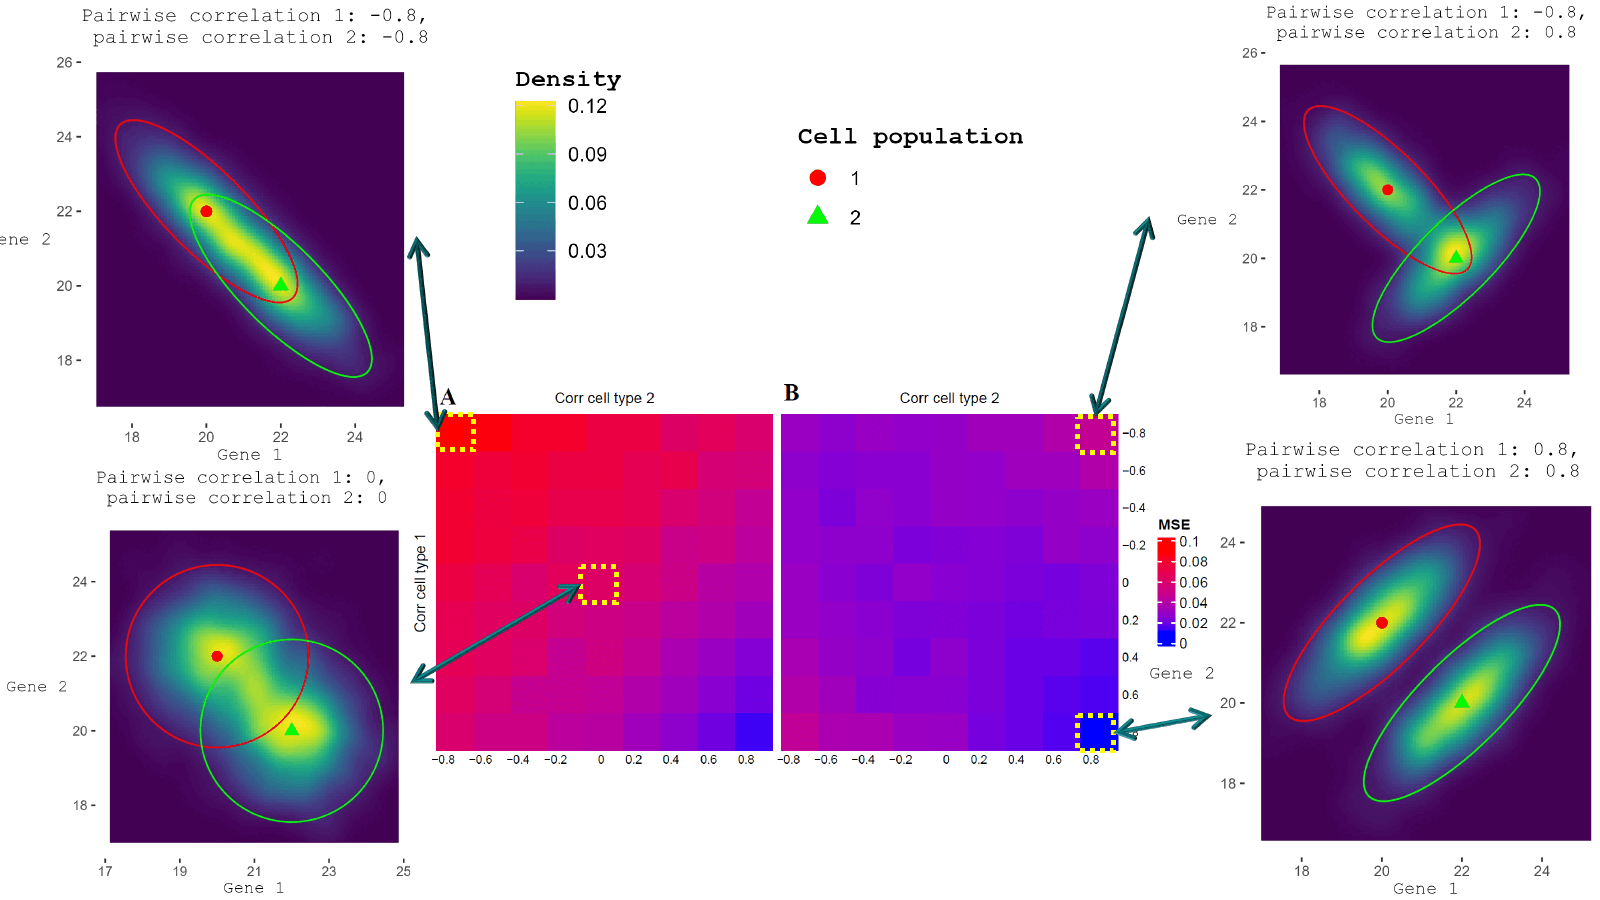
\includegraphics[width=0.9\textwidth]{
            deconvolution_Heatmap_full.png
        }
        \caption{We used the package \CRANpkg{ComplexHeatmap} to display the mean
        square error (MSE) of the estimated cell ratios, comparing the NNLS
        output, as implemented in the DeconRNASeq algorithm (\cite{gongDeconRNASeqStatisticalFramework2013}),
        in Panel \textbf{A}, with our newly implemented DeCovarT algorithm, in Panel
        \textbf{B}. The lower the MSE, the least noisy and biased the estimates.
        In addition, we added the two-dimensional density plot for the
        intermediate scenario, for which each population is parameterised by a diagonal
        covariance matrix, and the most extreme scenarios (those with the highest
        correlation between genes). The ellipsoids represent for each cell population
        the $95\%$ confidence region and the red spherical icon and the green triangular
        icon represent respectively the centroids (average expression of gene 1
        and gene 2) of cell population 1 and cell population 2.}
        \label{fig:mse-complex_heatmap}
    \end{figure}

    To evaluate the biological and statistical interest of \texttt{DeCovarT}, we
    then expand the simulation framework, by encompassing a larger number of cell
    types, genes, and testing the sensitivity of the model by voluntarily including
    noise in the benchmark evaluation.

    \subsubsection{Scaling numerical simulations using methods for generating
    synthetic networks}

    The general framework for generating realistic simulations of single-cell
    profiles while modelling interactions between genes comprises the following
    steps. First, generate the structure (skeleton of the graph, namely
    identfication of the edges's coverage), represented as a binary adjacency
    matrix. Then, shift the binary network into a weighted structure, with different
    interaction weights between genes (as available in a precision matrix),
    normalised between -1 and 1 -> each cell population exhibits its own
    distribution profile, parametrised by the simulated network structure.
    Finally, reflect the heteroeignity of cell composition in biological tissues
    by drawing cellular proportions from a Dirichlet distribution.

    \paragraph{Network generation}

    Un vaste pan de la littérature explored the generation of random and synthetic
    networks, each lying with its own assumptions. The most popular approaches are
    the Erdös-Rényi model (no particular structure), the preferential attachment
    model wich assumes a scale-free distribution of the degree of the network, and
    affiliation model, in which local structures prevail (see details in \ref{sec-synthetic-network}).
    However, all these models return a binary adjacency matrix, encoding only for
    the presence or absence of an interaction.

    The advantage of precision matrices precisely lies in the possibility of weighting
    edges by the strength of interaction, a higher absolute value depicting a
    stronger regulatory effect. Besides, the precision matrix should have the
    same sparsity level as the adjacency matrix, while being positive-definite.
    Inspiring from \cite{chiquetVariationalInferenceSparse2018} and \CRANpkg{huge},
    we enforce these two constraints with
    \ref{eq-affine-spectrum-transformation}:

    \begin{equation}
        \tilde{\boldsymbol{\Omega}}= \boldsymbol{A}\times v, \quad \boldsymbol{\Omega}
        = \tilde{\boldsymbol{\Omega}}+ \diag \left( \Bigg |\min \left( \text{Spectrum}
        {\left(\tilde{\boldsymbol{\Omega}}\right)}\right)\Bigg | + u \right) \label{eq-affine-spectrum-transformation}
    \end{equation}

    with $u$ and $v$ two scalar hyperparameters controlling the degree of connectivity
    in the graph. Precisely, $v$ controls the magnitude of the interactions,
    with higher $v$ inducing larger off-diagonal terms, while the second term of
    the equation $\diag \left(\min \left( |\Spectrum{\left(\tilde{\boldsymbol{\Omega}}\right)}
    | \right) + u \right)$ guarantees the strict positiveness of the matrix (see
    \ref{supp-thm-affine}). Accordingly, a fine balance must be found between the
    two hyperparameters, with a smaller $v$ implying a more diagonal and well-conditioned
    matrix, while a larger $v$ implies a stronger domination of the off-diagonal,
    interaction terms, and a larger spreading out of the spectrum.

    \todo{add visual with eigenvalues plots to demonstrate affine invariance of the spectrum}

    Of note, we would have considered other simualtion framework sfor generating
    interesting Gaussian distirbution scenarios. For instance, the Toeplitz
    sructure, modelling an exponetial decay with distance beween variables, is
    commonly used for generating structured covariance matricees. Indeed, it"s
    controlled by a single paramter $\rho$, making it highly interpretable, and
    easy to compute with the Cholesky decomposition. However, since its primary
    focus is on the covariance, the framework can only be used to encode local dependencies
    (and not global, accounting for all higher-order interactions, as for the
    precision matrix) \cite{batardiereEvaluatingParameterUncertainty2024,ogierduterrailFedECAFederatedExternal2025}.

    The \CRANpkg{mixSim} package, developed by \cite{melnykovMixSimPackageSimulating2012},
    and the \CRANpkg{clusterGeneration}, developed by
    \cite{qiuSeparationIndexPartial2006}, are other interesting alternatives for
    generating random clusters of cell populations, each modelled by a
    multivariate Gaussian distributions. However, \CRANpkg{mixSim} plays on the global
    level of overlap between cell-type specific distributions, while \CRANpkg{clusterGeneration}
    twists the level of degree separation between clusters, as quantified by a
    variant of the adjusted Rand Index.

    \subsection{Evaluation of robustness for DeCovarT}

    \todo{Sensitivity analyses, when the underlying distribution of counts is not Gaussian}

    \begin{itemize}
        \item Add Gaussian white noise as a white-error term

        \item Evaluate sensibility to other types of statistical distributions \cite{wangBulkTissueCell2019}

        \item Dropout rate, as in MuSiC \cite{wangBulkTissueCell2019}

        \item Incomplete single-cell references, with missing cell populations
            \cite{wangBulkTissueCell2019}

        \item Evaluate tolerance for different single-cell RNASeq protocols \cite{wangBulkTissueCell2019}
    \end{itemize}

    \section{Methods}

    \subsection{DeCovarT model set-up}

    In this section, we recall the paradigm underlying most deconvolution
    algorithms, relating bulk transcriptomic expression to cell type-specific
    gene expression. Indices are fixed throughout: gene $g=1,\ldots,G$;
    cell type $j=1,\ldots,J$; sample (subject) $i=1,\ldots,N$ (independence
    across samples). Column and row slices use the conventional dot notation
    ($\boldsymbol{\mu}_{\cdot j}$, $\boldsymbol{y}_{\cdot i}$). Analogously to
    MuSiC \cite{wangBulkTissueCell2019}, the signature stores
    \emph{cross-sample mean} profiles rather than a single draw of latent
    expression. Notations:
    \begin{itemize}
        \item $\boldsymbol{y}=(y_{gi})\in\mathbb{R}_{+}^{G\times N}$: bulk
            expression; $\boldsymbol{y}_{\cdot i}\in\mathbb{R}_{+}^{G}$ is the
            profile of sample $i$.

        \item $\boldsymbol{\mu}=(\mu_{gj})\in\mathbb{R}^{G\times J}$: mean
            signature; $\boldsymbol{\mu}_{\cdot j}\in\mathbb{R}^{G}$ is the
            mean profile of cell type $j$ (averaged over reference samples /
            cells, as in MuSiC).

        \item $\boldsymbol{p}=(p_{ji})\in\,]0,1[^{J\times N}$: unknown relative
            proportions; $\boldsymbol{p}_{\cdot i}\in\,]0,1[^{J}$ is the
            composition of sample $i$.

        \item $\boldsymbol{\Sigma}_{j}\in\mathbb{R}^{G\times G}$ and
            $\boldsymbol{\Theta}_{j}\equiv\boldsymbol{\Sigma}_{j}^{-1}$:
            covariance and precision of cell type $j$. Stacking over $j$
            yields third-order tensors of size $G\times G\times J$
            (one $G\times G$ network per cell type).
    \end{itemize}

    As in most traditional deconvolution models, bulk expression is the linear
    combination of mean cell-type profiles weighted by proportions
    (\ref{eq-linear-deconvolution}). The mean map is linear in
    $\boldsymbol{p}$. Each composition lies on the unit simplex
    (\ref{eq-simplex-constraint}), the setting of constrained
    least-squares simplicial regression
    \cite{tsagrisConstrainedLeastSquares2025}. The default open-simplex
    chart is the isometric log-ratio
    \cite{egozcueIsometricLogratioTransformations2003}; additive log-ratio
    maps remain available for comparison.
    \begin{equation}
        \label{eq-linear-deconvolution}
        \boldsymbol{y}=\boldsymbol{\mu}\,\boldsymbol{p}
        \quad\text{(equivalently }
        \boldsymbol{y}_{\cdot i}=\boldsymbol{\mu}\,\boldsymbol{p}_{\cdot i}
        \text{ for each }i\text{)}.
    \end{equation}
    \begin{equation}
        \label{eq-simplex-constraint}
        \begin{cases}
            \sum_{j=1}^{J} p_{ji}=1                      \\
            \forall j \in \widetilde{J}\quad p_{ji}\ge 0
        \end{cases}
        \qquad (i=1,\ldots,N).
    \end{equation}

    \subsection{Model assumptions}
    \label{subsec:model-assumptions-rank}

    In contrast to standard linear regression, DeCovarT relaxes
    \emph{exogeneity} by treating latent cell-type expression profiles as
    random rather than fixed. The closest published \emph{convolution} is
    DeMixT \cite{wangTranscriptomeDeconvolutionHeterogeneous2018} (and
    DeMix \cite{ahnDeMixDeconvolutionMixed2013}): frequentist Gaussian
    convolutions with an unknown tumour or stromal component, but
    gene-wise independent variances and no gene--gene residual network.
    DSection \cite{erkkilaProbabilisticAnalysisGene2010} is a
    \emph{Bayesian} univariate convolution (independent genes, Gibbs /
    Metropolis). Ogundijo and Wang
    \cite{ogundijoSequentialMonteCarlo2017} extend DSection by sequential
    Monte Carlo. DeCovarT keeps a closed reference
    $(\boldsymbol{\mu},\{\boldsymbol{\Sigma}_{j}\})$ and a frequentist
    multivariate convolution with sparse cell-type-specific
    $\boldsymbol{\Sigma}_{j}$; there is no unknown extra component.

    RNA-Sieve \cite{erdmann-phamLikelihoodbasedDeconvolutionBulk2021} is
    also a supervised, likelihood-based deconvolution, but of a different
    generative model. Writing their mean matrix $M$, mixing weights
    $\alpha$ and bulk $b$ for DeCovarT's $\boldsymbol{\mu}$,
    $\boldsymbol{p}$ and $\boldsymbol{y}$, they treat $b$ as the sum of
    $n$ independent cells and invoke a \emph{gene-wise} central-limit
    Gaussian whose variance $s_{g}^{2}(M,\alpha,S)$ depends on $\alpha$.
    They further model estimation error in $M$
    ($\varepsilon_{M,gk}\sim\mathcal{N}(0,s_{gk}/c_{k})$), an
    errors-in-variables correction of the design rather than a convolution
    of $J$ latent type profiles. Genes are taken as independent.
    DeCovarT instead convolves multivariate type profiles and treats
    $(\boldsymbol{\mu},\{\boldsymbol{\Sigma}_{j}\})$ as plug-in known.

    Latent profile $\boldsymbol{x}_{\cdot j}\in\mathbb{R}^{G}$ of cell type
    $j$ is multivariate Gaussian (\ref{eq-multivariate-gaussian}):
    \begin{equation}
        \label{eq-multivariate-gaussian}
        \DET(2\pi\boldsymbol{\Sigma}_{j})^{-\frac{1}{2}}
        \exp\!\Bigl(
        -\tfrac{1}{2}
        (\boldsymbol{x}_{\cdot j}-\boldsymbol{\mu}_{\cdot j})^{\top}
        \boldsymbol{\Theta}_{j}
        (\boldsymbol{x}_{\cdot j}-\boldsymbol{\mu}_{\cdot j})
        \Bigr),
    \end{equation}
    with parameters:
    \begin{itemize}
        \item $\boldsymbol{\mu}_{\cdot j}$: mean purified transcriptomic
            profile of cell type $j$ (column of $\boldsymbol{\mu}$);

        \item $\boldsymbol{\Sigma}_{j}$: positive-definite covariance
            (Appendix~\ref{def:positive-definite}), recovered via its inverse
            with \texttt{gLasso}
            \cite{mazumderGraphicalLassoNew2011}. We set
            $\boldsymbol{\Theta}_{j}\equiv\boldsymbol{\Sigma}_{j}^{-1}$;
            after normalisation, off-diagonal entries are partial
            correlations. Null off-diagonals are treated as absent edges.
    \end{itemize}

    Plug-in estimates
    $\zeta_{j}=(\boldsymbol{\mu}_{\cdot j},\boldsymbol{\Sigma}_{j})$ yield
    known
    $\boldsymbol{\zeta}=(\boldsymbol{\mu},\{\boldsymbol{\Sigma}_{j}\}_{j=1}^{J})$
    with $\boldsymbol{\mu}=(\boldsymbol{\mu}_{\cdot j})_{j\in\widetilde{J}}$.
    Conditionally on $(\boldsymbol{\zeta},\boldsymbol{p}_{\cdot i})$, the bulk
    $\boldsymbol{y}_{\cdot i}$ is a Gaussian convolution
    (\ref{eq-conditional-multivariate-distribution}):
    \begin{equation}
        \boldsymbol{y}_{\cdot i}\,|\,(\boldsymbol{\zeta},\boldsymbol{p}_{\cdot i})
        \sim\mathcal{N}_{G}\!\bigl(
        \boldsymbol{\mu}\,\boldsymbol{p}_{\cdot i},\,
        \textstyle\sum_{j=1}^{J}p_{ji}^{2}\boldsymbol{\Sigma}_{j}
        \bigr)
        \label{eq-conditional-multivariate-distribution}
    \end{equation}
    The directed graphical models associated with this framework are shown in
    Fig.~\ref{fig:DAG-model}: panel~\textbf{a} recalls the classical linear
    deconvolution template; panel~\textbf{b} is the unconstrained DeCovarT
    generative model; panel~\textbf{c} adds the regularised soft-max mapping
    $\boldsymbol{\psi}$ that enforces the unit-simplex constraint on
    $\boldsymbol{p}$. Classical OLS and Gauss--Markov reminders (Article length)
    are deferred to the package vignette
    \texttt{Beyond-OLS}.

    \begin{figure}[t]
        \centering
        % TikZ–bayesnet DAGs for DeCovarT (input from main.tex)
% Panel (a): linear gold-standard; (b) unconstrained; (c) constrained
% Use explicit \draw (not bayesnet \edge) to avoid nullfont `;' warnings.
\tikzset{
  param/.style={
      rectangle, draw=black, thick, minimum size=18pt, inner sep=2pt,
      font=\small
    },
  detcirc/.style={
      circle, draw=black, dashed, thick, fill=white, minimum size=22pt,
      inner sep=1pt, font=\small
    },
  obsdashed/.style={
      circle, draw=black, dashed, thick, fill=gray!30, minimum size=22pt,
      inner sep=1pt, font=\small
    },
  dagplate/.style={
      draw, dashed, thick, rounded corners=2pt, inner sep=8pt
    },
  eqtext/.style={font=\scriptsize, text=black, align=center}
}

% -------------------- (a) Linear model --------------------
\begin{tikzpicture}[x=1.2cm, y=1.15cm, >=stealth]
  \node[param] (p) at (0, 1.2) {$\boldsymbol{p}_{\cdot i}$};
  \node[param] (sig) at (0, 0) {$\sigma_{i}$};
  % Wider gutters: left (params → gene plate) and right (gene plate → $\mu_{gj}$)
  \node[obs] (y) at (3.0, 0.6) {$y_{gi}$};
  \node[param] (x) at (6.2, 0.6) {$\mu_{gj}$};

  \draw[->] (p) -- (y);
  \draw[->] (sig) -- (y);
  \draw[->] (x) -- (y);

  \node[above=0.35cm of y, eqtext]
  (ylik) {%
    $y_{gi\,|\,\cdot}
    \sim\mathcal{N}\!\bigl(\sum_{j}\mu_{gj}p_{ji},\,\sigma_{i}^{2}\bigr)$%
  };

  \plate[dagplate, inner sep=12pt]{plateG}{(y)(ylik)}{$g\in\{1,\ldots,G\}$};
  \plate[dagplate, inner sep=16pt, inner xsep=22pt]
    {plateN}{(p)(sig)(plateG)}{$i\in\{1,\ldots,N\}$};

  \node[font=\footnotesize\bfseries, text=black, below=0.75cm of plateN.south]
  {\textbf{a} Standard linear deconvolution (gold-standard template).};
\end{tikzpicture}

\vspace{1.6em}

% -------------------- (b) Unconstrained DeCovarT --------------------
\begin{tikzpicture}[x=1.1cm, y=1.05cm, >=stealth, font=\small]
  \node[detcirc] (p) at (0, 0.9) {$\boldsymbol{p}_{\cdot i}$};
  \node[obsdashed] (y) at (0, -0.6) {$\boldsymbol{y}_{\cdot i}$};
  \draw[->, dashed] (p) -- (y);

  \node[latent] (xj) at (4.2, 0.9) {$\boldsymbol{x}_{\cdot j}$};
  \node[param] (mu) at (3.3, 2.3) {$\boldsymbol{\mu}_{\cdot j}$};
  \node[param] (Sj) at (5.1, 2.3) {$\boldsymbol{\Sigma}_{j}$};
  \draw[->] (mu) -- (xj);
  \draw[->] (Sj) -- (xj);
  \draw[->, dashed] (xj) -- (y);

  \node[above=0.25cm of xj, eqtext]
  {$\boldsymbol{x}_{\cdot j}\sim\mathcal{N}_{G}(\boldsymbol{\mu}_{\cdot j},
    \boldsymbol{\Sigma}_{j})$};

  \node[left=0.12cm of y, eqtext, align=right]
  {%
    $\boldsymbol{y}_{\cdot i\,|\,\cdot}\sim\mathcal{N}_{G}\!\bigl(
    \boldsymbol{\mu}\boldsymbol{p}_{\cdot i},
    \sum_{j}p_{ji}^{2}\boldsymbol{\Sigma}_{j}\bigr)$%
  };

  \node[eqtext] at ($(xj)!0.55!(y)+(0.25,-0.3)$)
  {$\boldsymbol{y}_{\cdot i}=\boldsymbol{\mu}\boldsymbol{p}_{\cdot i}$};

  \plate[dagplate]{plateI}{(p)(y)}{$i\in\{1,\ldots,N\}$};
  \plate[dagplate]{plateJ}{(xj)(mu)(Sj)}{$j\in\{1,\ldots,J\}$};

  \node[font=\footnotesize\bfseries, text=black,
    below=0.75cm of plateI.south west, anchor=north west]
  {\textbf{b} Unconstrained DeCovarT generative model.};
\end{tikzpicture}

\vspace{1.6em}

% -------------------- (c) Constrained DeCovarT --------------------
\begin{tikzpicture}[x=1.1cm, y=1.0cm, >=stealth, font=\small]
  \node[latent] (th) at (0, 2.1) {$\boldsymbol{\rho}_{i}$};
  \node[detcirc] (p) at (0, 0.9) {$\boldsymbol{p}_{\cdot i}$};
  \node[obsdashed] (y) at (0, -0.55) {$\boldsymbol{y}_{\cdot i}$};
  \draw[->] (th) -- (p);
  \draw[->, dashed] (p) -- (y);

  \node[latent] (xj) at (4.2, 0.9) {$\boldsymbol{x}_{\cdot j}$};
  \node[param] (mu) at (3.3, 2.3) {$\boldsymbol{\mu}_{\cdot j}$};
  \node[param] (Sj) at (5.1, 2.3) {$\boldsymbol{\Sigma}_{j}$};
  \draw[->] (mu) -- (xj);
  \draw[->] (Sj) -- (xj);
  \draw[->, dashed] (xj) -- (y);

  \node[left=0.12cm of y, eqtext, align=right]
  {%
    $\boldsymbol{y}_{\cdot i\,|\,\cdot}\sim\mathcal{N}_{G}\!\bigl(
    \boldsymbol{\mu}\boldsymbol{p}_{\cdot i},
    \sum_{j}p_{ji}^{2}\boldsymbol{\Sigma}_{j}\bigr)$%
  };

  \plate[dagplate]{plateIc}{(th)(p)(y)}{$i\in\{1,\ldots,N\}$};
  \plate[dagplate]{plateJc}{(xj)(mu)(Sj)}{$j\in\{1,\ldots,J\}$};

  \node[font=\footnotesize\bfseries, text=black,
    below=0.75cm of plateIc.south west, anchor=north west]
  {\textbf{c} Constrained DeCovarT (regularised soft-max on the simplex).};
\end{tikzpicture}

\vspace{1.2em}

        \caption[DAG models for linear and DeCovarT deconvolution]{%
            Directed graphical models (plate notation), following the conventions
            of \href{https://revbayes.github.io/tutorials/intro/graph_models.html}{RevBayes}.
            Shaded nodes are observed; square nodes are fixed (plug-in) parameters;
            dashed circles denote deterministic or constrained quantities.
            \textbf{a}~Gold-standard linear model
            $y_{gi\,|\,\cdot}\sim\mathcal{N}(\sum_{j}\mu_{gj}p_{ji},
            \sigma_{i}^{2})$.
            \textbf{b}~Unconstrained DeCovarT convolution
            $\boldsymbol{y}_{\cdot i\,|\,\cdot}\sim\mathcal{N}_{G}(\boldsymbol{\mu}
            \boldsymbol{p}_{\cdot i},\sum_{j}p_{ji}^{2}\boldsymbol{\Sigma}_{j})$ with
            $\boldsymbol{x}_{\cdot j}\sim\mathcal{N}_{G}(\boldsymbol{\mu}_{\cdot j},
            \boldsymbol{\Sigma}_{j})$.
            \textbf{c}~Constrained DeCovarT: unconstrained coordinates
            $\boldsymbol{\rho}_{i}\in\mathbb{R}^{J-1}$ are mapped to the open
            simplex by the $C^{2}$-diffeomorphism
            $\boldsymbol{\psi}:\boldsymbol{\rho}\mapsto\boldsymbol{p}$ with
            $p_{j}=e^{\rho_{j}}/(\sum_{k<J}e^{\rho_{k}}+1)$ for $j<J$,
            $p_{J}=1/(\sum_{k<J}e^{\rho_{k}}+1)$, and inverse
            $\boldsymbol{\psi}^{-1}(\boldsymbol{p})=
            \bigl(\ln(p_{j}/p_{J})\bigr)_{j<J}$
            (Eq.~\ref{eq-mapping-function}).
            Variability is attributed to latent covariates
            $\boldsymbol{x}_{\cdot j}$.%
        }
        \label{fig:DAG-model}
    \end{figure}

    In the next section, we provide an explicit formula of the log-likelihood of
    our probabilistic framework, its gradient and hessian, which in turn can be
    used to retrieve the MLE of our distribution.

    \subsection{Derivation of the log-likelihood}

    From \ref{eq-conditional-multivariate-distribution}, the conditional log-likelihood
    is readily computed and given by
    \ref{eq-loglikelihood-multivariate-gaussian}:

    \begin{equation}
        \ell_{\boldsymbol{y} | \boldsymbol{\zeta}}(\boldsymbol{p})=C + \frac{1}{2}\log
        \left(\DET \left(\sum_{j=1}^{J} p_{j}^{2}\boldsymbol{\Sigma}_{j}\right)^{-1}\right
        ) - \frac{1}{2}(\boldsymbol{y}- \boldsymbol{\mu}\boldsymbol{p})^{\top} \left
        (\sum_{j=1}^{J} p_{j}^{2}\boldsymbol{\Sigma}_{j}\right)^{-1}(\boldsymbol{y}
        - \boldsymbol{\mu}\boldsymbol{p}) \label{eq-loglikelihood-multivariate-gaussian}
    \end{equation}

    Both the log-determinant and the Mahalanobis residual carry the factor
    $\frac{1}{2}$ of the Gaussian log-density
    (\ref{eq-conditional-multivariate-distribution}). Keeping that factor is
    what makes the score and Hessian derived below consistent with the
    expected Fisher information used for Wald inference in
    \ref{subsec:asymptotic-inference}: taking expectations of
    \ref{eq-hessian-log-likelihood-unconstrained} under the generative model
    returns $\mathcal{I}(\boldsymbol{p})$ exactly.

    \subsection{First and second-order derivation of the unconstrained DeCovarT
    log-likelihood function}
    \label{subsec:uncontrained-optimisation}

    The stationary points of a function and notably maxima, are given by the roots
    (the values at which the function crosses the $x$-axis) of its gradient, in
    our context, the vector: $\nabla \ell: \RR^{J} \to \RR^{J}$ evaluated at
    point $\nabla \ell (\boldsymbol{p}): ]0, 1[^{J} \to \RR^{J}$. Since the computation
    is the same for any cell ratio $p_{j}$, we give an explicit formula for only
    one of them (\ref{eq-derivative-log-likelihood-unconstrained}):

    \begin{equation}
        \label{eq-derivative-log-likelihood-unconstrained}
        \begin{split}
            \frac{\partial \ell_{\boldsymbol{y} | \boldsymbol{\zeta}}(\boldsymbol{p})}{\partial
            p_{j}}=&\scriptstyle \frac{1}{2}\frac{\partial \log\left(\DET(\boldsymbol{\Theta})\right)}{\partial
            p_{j}}-\frac{1}{2}\left[\frac{\partial (\boldsymbol{y}- \boldsymbol{\mu}\boldsymbol{p})^{\top}}{\partial
            p_{j}}\boldsymbol{\Theta}(\boldsymbol{y}- \boldsymbol{\mu}\boldsymbol
            {p}) + (\boldsymbol{y}- \boldsymbol{\mu}\boldsymbol{p})^{\top}\frac{\partial\boldsymbol{\Theta}}{\partial
            p_{j}}(\boldsymbol{y}- \boldsymbol{\mu}\boldsymbol{p}) + (\boldsymbol
            {y}- \boldsymbol{\mu}\boldsymbol{p})^{\top}\boldsymbol{\Theta}\frac{\partial
            (\boldsymbol{y} - \boldsymbol{\mu} \boldsymbol{p})}{\partial p_{j}}\right
            ]\\
            =&\scriptstyle -\frac{1}{2}\Tr \left(\boldsymbol{\Theta}\frac{\partial
            \boldsymbol{\Sigma}}{\partial p_{j}}\right) - \frac{1}{2}\left[ - \boldsymbol
            {\mu}_{\cdot j}^{\top}\boldsymbol{\Theta}(\boldsymbol{y}- \boldsymbol{\mu}
            \boldsymbol{p}) - (\boldsymbol{y}- \boldsymbol{\mu}\boldsymbol{p})^{\top}
            \Theta\frac{\partial \Sigma}{\partial p_{j}}\Theta(\boldsymbol{y}- \boldsymbol
            {\mu}\boldsymbol{p}) - (\boldsymbol{y}- \boldsymbol{\mu}\boldsymbol{p}
            )^{\top}\boldsymbol{\Theta}\boldsymbol{\mu}_{\cdot j}\right] \\
            =&\textcolor{purple}{-p_j \Tr \left(\boldsymbol{\Theta}\boldsymbol{\Sigma}_j\right)
            }+ \textcolor{blue}{(\boldsymbol{y} - \boldsymbol{\mu} \boldsymbol{p})^\top\boldsymbol{\Theta}
            \boldsymbol{\mu}_{\cdot j}}\, + \textcolor{orange}{p_j (\boldsymbol{y} -
            \boldsymbol{\mu} \boldsymbol{p})^\top\boldsymbol{\Theta} \Sigma_j
            \boldsymbol{\Theta} (\boldsymbol{y} - \boldsymbol{\mu} \boldsymbol{p})
            }
        \end{split}
    \end{equation}

    Since the solution to $\nabla \left( \ell_{\boldsymbol{y} | \boldsymbol{\zeta}}
    (\boldsymbol{p}) \right) =0$ is not closed, we had to approximate the MLE
    using iterated numerical optimisation methods. Some of them, such as the
    Levenberg–Marquardt algorithm, require a second-order approximation of the function,
    which needs the computation of the Hessian matrix. Deriving once more \ref{eq-derivative-log-likelihood-unconstrained}
    yields the Hessian matrix, $\mathbf{H}\in \mathcal{M}_{J \times J}$ is given
    by:
    \begin{equation}
        \label{eq-hessian-log-likelihood-unconstrained}
        \begin{aligned}
            \mathbf{H}_{i,i} & = \frac{\partial^2 \ell}{\partial^2 p_i}= \textcolor{purple}{-\Tr \left(\boldsymbol{\Theta}\boldsymbol{\Sigma}_i\right) + 2p_i^2 \Tr \left(\left(\boldsymbol{\Theta}\boldsymbol{\Sigma}_i\right)^2\right)}\textcolor{blue}{-2p_i(\boldsymbol{y} - \boldsymbol{\mu} \boldsymbol{p})^\top\boldsymbol{\Theta} \boldsymbol{\Sigma}_i \boldsymbol{\Theta} \boldsymbol{\mu}_{\cdot i}\, - \boldsymbol{\mu}_{\cdot i}^\top\boldsymbol{\Theta} \boldsymbol{\mu}_{\cdot i}}\, -        \\
                             & \textcolor{orange}{2p_i (\boldsymbol{y} - \boldsymbol{\mu} \boldsymbol{p})^\top \boldsymbol{\Theta}\boldsymbol{\Sigma}_i\boldsymbol{\Theta}\boldsymbol{\mu}_{\cdot i} \, - (\boldsymbol{y} - \boldsymbol{\mu} \boldsymbol{p})^\top\boldsymbol{\Theta} \left(4p_i^2 \boldsymbol{\Sigma}_i \boldsymbol{\Theta} \boldsymbol{\Sigma}_i - \boldsymbol{\Sigma}_i \right)\boldsymbol{\Theta} (\boldsymbol{y} - \boldsymbol{\mu} \boldsymbol{p})}, \quad i \in \widetilde{J} \\
            \mathbf{H}_{i,j} & = \frac{\partial^2 \ell}{\partial p_i \partial p_j}= \textcolor{purple}{2p_j p_i \Tr \left(\boldsymbol{\Theta}\boldsymbol{\Sigma}_j \boldsymbol{\Theta}\boldsymbol{\Sigma}_i \right)}\textcolor{blue}{-2p_i(\boldsymbol{y} - \boldsymbol{\mu} \boldsymbol{p})^\top\boldsymbol{\Theta} \boldsymbol{\Sigma}_i \boldsymbol{\Theta} \boldsymbol{\mu}_{\cdot j} - \boldsymbol{\mu}_{\cdot i}^\top\boldsymbol{\Theta} \boldsymbol{\mu}_{\cdot j}}\, -                                \\
                             & \textcolor{orange}{2p_j (\boldsymbol{y} - \boldsymbol{\mu} \boldsymbol{p})^\top \boldsymbol{\Theta}\boldsymbol{\Sigma}_j\boldsymbol{\Theta} \boldsymbol{\mu}_{\cdot i}\, - 4p_ip_j(\boldsymbol{y} - \boldsymbol{\mu} \boldsymbol{p})^\top\boldsymbol{\Theta}\boldsymbol{\Sigma}_i \boldsymbol{\Theta} \boldsymbol{\Sigma}_j \boldsymbol{\Theta} (\boldsymbol{y} - \boldsymbol{\mu} \boldsymbol{p})}, \quad (i,j) \in \widetilde{J}^{2}, i \neq j
        \end{aligned}
    \end{equation}
    in which the coloured sections pair one by one with the corresponding coloured
    sections of the gradient, given in
    \ref{eq-derivative-log-likelihood-unconstrained}.

    Matrix calculus can largely ease the derivation of complex algebraic
    expressions, thus we remind in Appendices A.1 and A.2 relevant matrix properties
    and derivations. The numerical consistency of these derivatives was asserted
    with the \CRANpkg{numDeriv} package, using the more stable Richardson’s
    extrapolation

    However, the explicit formulas for the gradient and the hessian matrix of the
    log-likelihood function, given in
    \ref{eq-derivative-log-likelihood-unconstrained} and
    \ref{eq-hessian-log-likelihood-unconstrained} respectively, do not take into
    account the simplex constraint assigned to the ratios. While some
    optimisation methods use heuristic methods to solve this problem, we consider
    alternatively a reparametrised version of the problem, detailed
    comprehensively in Appendix A.3.

    \section{Discussion}

    While other approaches, such as \texttt{DeMix} and \texttt{DeMixT}, enabled,
    using a sound statistical framework, to jointly estimate cellular portions
    and distributions of gene expression per sample and cell population, \texttt{DeCovarT}
    is the first deconvolution algorithm which explicitly handles the unit-simplex
    constraint, addressing the intrinsic compositional nature of cellular composition,
    while integrating interactions between genes.

    Through extensive numerical simulations, playing on varying levels of gene

    Hence, it provides a strong basis to further derive statistical tests to assert
    whether the proportion of a given cell population differs significantly between
    two distinct biological conditions.

    \subsection{Limitations and outlook}

    The present estimator is a closed-reference Gaussian convolution: every
    abundant cell type is assumed to appear as a column of $\boldsymbol{\mu}$,
    bulk and reference profiles are taken to lie on a compatible expression
    scale, and sample-level covariates, sequencing exposure, cell-type
    transcriptome size and condition-dependent shifts in
    $\boldsymbol{\mu}_{\cdot j}$ are not modelled. Graphical-lasso estimates of
    $\boldsymbol{\Theta}_{j}$ additionally shrink non-zero partial correlations.
    These restrictions motivate the extensions below; a longer catalogue with
    equations is given in the package perspectives vignette.

    DeCovarT is not ordinary least squares. Cell-type covariances enter the
    residual law \(\boldsymbol{\Sigma}(\boldsymbol{p}_{\cdot i})\) and cannot be
    treated as extra columns of \(\boldsymbol{\mu}\). There is therefore no
    formula / \texttt{lm} interface, and no \texttt{predict()} method for
    forecasting bulk transcriptomes. Gene-wise affine standardisation
    (z-scoring \(\boldsymbol{y}_{\cdot i}\), \(\boldsymbol{\mu}\) and
    \(\boldsymbol{\Sigma}_{j}\) with the same centre and scale) is equivariant
    for \(\hat{\boldsymbol{p}}\)
    (\ref{pr:decovart-affine-equivariance}); logarithms and
    per-cell-type or per-sample transforms are not. Wald intervals use the
    expected Fisher information of the convolution mapped through the ALR
    (\ref{pr:decovart-expected-fisher}). A systematic study of CPM / log2
    normalisation, optimiser tolerance, and scaling with \(G\), \(J\) and
    signature overlap is left to a later benchmark.

    RNA-Sieve reports Wald regions from the inverse Fisher information of
    its gene-wise CLT likelihood, and a Godambe sandwich when protocol
    shift takes the truth outside the model family
    \cite{erdmann-phamLikelihoodbasedDeconvolutionBulk2021}. DeCovarT's
    analogue of the first is
    (\ref{pr:decovart-expected-fisher}); it is not calibrated on a simplex
    face, where the chi-bar-square likelihood-ratio test and a restricted
    parametric bootstrap are required. A Godambe correction would be the
    natural sandwich if the multivariate convolution itself is
    misspecified. RNA-Sieve's noisy-$M$ term is the likelihood analogue of
    resampling the reference; DeCovarT currently keeps
    $\boldsymbol{\mu}$ and $\boldsymbol{\Sigma}_{j}$ plug-in and
    propagates that uncertainty by a donor- or cell-level bootstrap. The
    package vignette on MLE properties compares the two generative models
    in notation aligned with (\ref{eq-linear-deconvolution}).

    Real-data evaluation should start from matched flow-cytometry / bulk
    RNA-seq panels such as the Kassandra benchmark
    \cite{zaitsevPreciseReconstructionTME2022}, which already compares EPIC
    \cite{racleSimultaneousEnumerationCancer2017}, CIBERSORT
    \cite{newmanRobustEnumerationCell2015}, CIBERSORTx
    \cite{newmanDeterminingCellType2019}, quanTIseq \cite{finotello_etal19}
    and ABIS \cite{monacoRNASeqSignaturesNormalized2019}.

    \paragraph{Observation laws and sample-level CTS.}
    DeCovarT is a continuous, frequentist convolution with plug-in
    $\boldsymbol{\mu}$ and $\boldsymbol{\Sigma}_{j}$. Discrete alternatives include
    multinomial--Dirichlet purification (ISOpureR, BayesPrism)
    \cite{anghelISOpureRImplementationComputational2015,chuCellTypeGeneExpression2022}
    and Poisson / Poisson--log-normal count models
    \cite{chiquetPoissonLognormalModelVersatile2021}. BLADE replaces the
    Gaussian by a gene-wise log-normal convolution and jointly infers
    cell-type-specific (CTS) expression
    \cite{andrade-barbosaBayesianLogNormalDeconvolution2021}. A Bayesian CTS
    step for DeCovarT would recover $\boldsymbol{x}_{\cdot j,i}$ given
    $\boldsymbol{y}_{\cdot i}$ and $\boldsymbol{p}_{\cdot i}$ under the existing
    multivariate likelihood---the univariate analogue is DSection
    \cite{erkkilaProbabilisticAnalysisGene2010}. Isoform-level signatures
    $\boldsymbol{\mu}^{\mathrm{iso}}\in\mathbb{R}^{T\times J}$ can further
    exploit differential transcript usage
    \cite{heilingEstimatingCellTypeComposition2023}.

    \paragraph{Covariates, unknown types, and RNA--cell uncoupling.}
    Sample-level covariates $\boldsymbol{z}_{i}$ cannot be appended as extra
    columns of $\boldsymbol{\mu}$. They may modulate cell-state moments
    $\boldsymbol{\mu}_{j}(\boldsymbol{z}_{i})$ (as in MuSiC2, which drops
    condition-specific genes while remaining closed-reference)
    \cite{fanMusic2CellTypeDeconvolution2022} or the ALR coordinates of
    $\boldsymbol{p}_{\cdot i}$. Incomplete references require an explicit unknown
    component $p_{u,i}\boldsymbol{u}_{i}$ or a signature adjustment: DICEPro
    wraps existing engines when columns of $\boldsymbol{\mu}$ are missing
    \cite{baWhenLessNot2026}; BayICE adds a Bayesian unknown type with
    spike-and-slab selection \cite{taiBayiceBayesianHierarchicalModel2021};
    EPIC already includes an uncharacterised compartment
    \cite{racleSimultaneousEnumerationCancer2017}. Independently, RNA mass
    fractions differ from cytometric cell fractions whenever transcriptome
    sizes $r_{j}$ are heterogeneous. EPIC and quanTIseq apply a
    post-correction $\hat p_{j}^{\ast}\propto\hat p_{j}/r_{j}$ with measured
    or proxied $r_{j}$
    \cite{racleSimultaneousEnumerationCancer2017,finotello_etal19,luTranscriptomeSizeMatters2025};
    MMAD instead estimates $r_{j}$ as an extra parameter, so the
    mixture is no longer linear \cite{liebnerMMADMicroarrayMicrodissection2014}.

    \paragraph{Weighted and generalised least squares.}
    DWLS down-weights noisy genes by a diagonal $W$
    \cite{tsoucasAccurateEstimationCelltype2019}. Ingesting those weights
    into BayesPrism is currently a strong joint $\boldsymbol{p}$+CTS combination
    \cite{zhangIntegratedInferenceCellularCompositions2026}; the DeCovarT
    analogue is a weighted convolution
    $\boldsymbol{y}^{\star}=W^{1/2}\boldsymbol{y}$,
    $\boldsymbol{\Sigma}_{j}^{\star}=W^{1/2}\boldsymbol{\Sigma}_{j}W^{1/2}$
    (\ref{th:generalized-least-squares-estimate}).
    Generalised least squares with a \emph{global} residual covariance
    $\Sigma=J^{-2}\sum_{j}\boldsymbol{\Sigma}_{j}$ (equi-balanced $p_{j}=1/J$) is
    a simpler competitor that ignores cell-type-specific networks;
    cellGeometry estimates such a gene-level covariance from cross-sample
    variances \cite{lauCellGeometryUltrafastSinglecell2026}. Lineage trees
    add parent--child constraints on $\boldsymbol{p}$
    \cite{wangBulkTissueCell2019}; elastic-net methods such as DCQ target
    which types \emph{change} over time rather than a static simplex
    snapshot \cite{altboumDigitalCellQuantification2014}; EnsDeconv fuses
    several bulk engines into one $\hat{\boldsymbol{p}}$
    \cite{caiRobustAccurateEstimation2022}. Each spot of a spatial assay is
    the same mixture with its own $\boldsymbol{p}(s)$
    \cite{gaspard-boulincCelltypeDeconvolutionMethods2025}.

    \section{Code availability}

    All analyses were performed on ... high-performance computing infrastructure
    using StdEnv/2020. Core statistical analyses and deconvolution bench-marking
    were conducted in R (version 4.3.1), employing the following key packages:
    Seurat (v 4.3.0) for single-cell data processing; limma (v3.58.1), edgeR (v4.0.16),
    and DESeq2 (v1.42.1) for differential expression and discordant-gene
    filtering; lme4 (v1.1.35.5) and lmerTest (v3.1.3) for mixed-effects
    modelling; and tidyverse (v2.0.0) for data manipulation. Fifteen
    deconvolution methods were benchmarked, including EPIC (v1.1.7), FARDEEP (v1.0.1),
    MuSiC (v1.0.0), MuSiC2 (v0.1.0), BisqueRNA (v1.0.5), BayesPrism (v2.2.2), DWLS,
    hspe (v0.1), TOAST (v1.16.0), CSC-DRNA (v1.0.3), CSsingle (v0.1.0), DeconRNASeq
    (v1.44.0), and PREDE (v1.2.1). CIBERSORTx deconvolution was performed via its
    web interface (https://cibersortx.stanford.edu/). Additional methods,
    AutoGeneS and GEDIT, were implemented in Python (version 3.10) with numpy,
    pandas, and scipy.

    Visualisation was performed using ggplot2 (v3.5.1), patchwork (v1.2.0), and cowplot
    (v1.1.3). To ensure reproducibility, all random seeds were fixed.

    The package used to generate the simulations and infer ratios from virtual or
    real biological mixtures with the DeCovarT algorithm is implemented on Github
    \href{https://github.com/bastienchassagnol/DeCovarT}{DeCovarT}.

    \section{Author contributions}

    B.C.\ conceived the method, implemented the \texttt{DeCovarT} package,
    designed the simulation studies, and wrote the manuscript. M.P.\ contributed
    equally to the methodological development and manuscript drafting.
    M.A.C.\ contributed to the benchmarking of gene-regulatory-network inference
    techniques used in the synthetic scenarios. G.N., E.B.\ and A.B.\ jointly
    supervised the work and revised the manuscript. All authors approved the
    final version.

    \section{Conflicts of interest}

    The authors declare no conflict of interest.

    \section{Acknowledgments}

    We thank Boris Hejblum for advice on computational performance and numerical
    precision, notably the use of the log-sum-exp trick for evaluating the
    additive logistic (softmax) map and its derivatives. We thank Kalidou~Ba for
    suggestions on pre-processing and normalisation of bulk and single-cell omics
    inputs to deconvolution algorithms. We thank Annesh~Pal for ideas on more
    realistic synthetic scenarios for DeCovarT, in particular the use of random
    graph models to generate richer topological structures for gene-regulatory
    networks.

    \backmatter

    \begin{appendices}
        \section{Synthetic network simulation}
        \label{sec-synthetic-network}

        The three most popular approaches for generating random, synthetic networks
        are:
        \begin{itemize}
            \item The Erdős–Rényi model was first described in \cite{barabasiEmergenceScalingRandom1999}:
                edges are generated independently between each pair of nodes
                with a fixed probability, leading to a homogeneous random graph.

            \item In the preferential attachment model (\cite{newmanStructureDynamicsNetworks2011,lima-mendezPowerfulLawPower2009}), nodes are iteratively added, favouring
                connection to the most well-connected nodes. This kind of
                framewrok is compliant with the scale-free network property, often
                looked for in biological systems, and resulting in the emergence
                of hubs. The degree distribution is notably given by a power-law.

            \item The affiliation model, also known as the stochastic block
                model (see \cite{hollandStochasticBlockmodelsFirst1983}), assumes
                a latent indicator variable assigning each node to a community.
                The generation of edges is then dependent on group membership, with
                sronger interactions within a given block.
        \end{itemize}

        \todo{add a drawing of these three approaches}

        \begin{theorem}[Invariance of the spectrum function by affine
        transformation]
            \label{supp-thm-affine}

            Let $X$ be any square matrix, and consider the affine transformation:

            \[
                Y = aX + bI
            \]

            with $a$ and $b$ positive scalars, and $I$ the identity matrix. Then,
            the eigenvectors of $\boldsymbol{Y}$ are the same as $\boldsymbol{X}$,
            and the eigenvalues are linearly transformed, shifted by $b$ and scaled
            by $a$ (larger range if $a$ is above 1).
        \end{theorem}

        \section{Optimisation and calculus}

        \subsection{Multivariate Gaussian reminders}
        \label{subsec:ols-assumptions}
        % Classical OLS / Gauss--Markov material lives in the package vignette
        % vignettes/Beyond-OLS.qmd (kept out of the Article word budget).

        \begin{definition}[Multivariate Gaussian distributions]
            \label{def:multivariate-gaussian} If random vector $\boldsymbol{X}$ of
            size $G$ follows a random multivariate Gaussian distribution,
            $\boldsymbol{X}\sim \mathcal{N}_{G}(\mu, \boldsymbol{\Sigma})$, then
            its distribution is given by:
            \begin{equation*}
                \DET(2\pi\Sigma)^{-\frac{1}{2}}\exp\left( -\frac{1}{2}(\boldsymbol
                {x}- \mu) \Sigma^{-1}(\boldsymbol{x}- \mu)^{\top}\right)
            \end{equation*}
            in which:
            \begin{itemize}
                \item $\mu=\boldsymbol{X}$ is the $G$-dimensional mean vector

                \item $\boldsymbol{\Sigma}$ is a $G\times G$ positive-definite \ref{def:positive-definite}
                    covariance matrix, whose diagonal terms, $\diag(\boldsymbol{\Sigma}
                    )=[(\VV{X_{i,j}}), \, \forall (i, j) \in \widetilde{G}^{2}, i
                    = j]^{\top}$ are the individual variances of each purified gene
                    transcript in population $j$ and off-diagonal terms,
                    $\boldsymbol{\Sigma}_{i,j}=\CC{X_{i}, X_{j}}, \, \forall (i,
                    j) \in \widetilde{G}^{2}, i \neq j$
                    are the covariance between variables. We note $\Theta=\Sigma^{-1}$,
                    the inverse of the covariance matrix, called the \textit{precision
                    matrix}.
            \end{itemize}
        \end{definition}

        \begin{remark}[Affine invariance property of multivariate GMMs]
            \label{pr:multivariate-affine-transformation}

            The two following properties hold for a multivariate Gaussian
            distribution:
            \begin{itemize}
                \item if $\boldsymbol{X}\sim \mathcal{N}_{G}( \mu, \boldsymbol{\Sigma}
                    )$, then $p\boldsymbol{X}$, with $p$ a constant, follows
                    itself a multivariate Gaussian distribution, given by:
                    $p\boldsymbol{X}\sim \mathcal{N}_{G} (p \mu, p^{2} \Sigma)$

                \item given two independent random vectors $\boldsymbol{X_1}\sim
                    \mathcal{N}_{G}(\mu_{1}, \boldsymbol{\Sigma_1})$ and $\boldsymbol
                    {X_2}\sim \mathcal{N}_{G}(\mu_{2}, \boldsymbol{\Sigma_2})$ following
                    a multivariate Gaussian distribution, then the random
                    variable $\boldsymbol{X_1}+ \boldsymbol{X_2}$ follows itself
                    the multivariate Gaussian distribution:
                    \begin{equation*}
                        X + Y \sim \mathcal{N}_{G} (\mu_{1} + \mu_{2}, \boldsymbol
                        {\Sigma_1}+ \boldsymbol{\Sigma_2})
                    \end{equation*}

                    By induction, this property generalises to the sum of \(J\) independent
                    random vectors of same dimension \(\RR^{G}\).
            \end{itemize}
        \end{remark}

        \begin{remark}[Equivariance of the DeCovarT MLE]
            \label{pr:decovart-affine-equivariance}

            DeCovarT is equivariant to any fixed, invertible, gene-wise affine
            transformation applied consistently to bulk expression, reference
            means and reference covariances. Such transformations therefore do
            not alter the theoretical proportion estimates, although they may
            affect numerical conditioning. Transformations estimated separately
            for each cell type or bulk sample are not equivalent and are not
            supported.

            Let \(D=\mathrm{diag}(s_{1},\ldots,s_{G})\) with \(s_{g}\neq 0\)
            and \(\boldsymbol{m}\in\mathbb{R}^{G}\). The gene-wise map
            \begin{equation*}
                \boldsymbol{y}^{\star}_{\cdot i}
                = D^{-1}(\boldsymbol{y}_{\cdot i}-\boldsymbol{m}),
                \quad
                \boldsymbol{\mu}^{\star}
                = D^{-1}(\boldsymbol{\mu}-\boldsymbol{m}\boldsymbol{1}_{J}^{\top}),
                \quad
                \boldsymbol{\Sigma}_{j}^{\star}
                = D^{-1}\boldsymbol{\Sigma}_{j} D^{-1}
            \end{equation*}
            preserves the linear convolution: because
            \(\boldsymbol{1}_{J}^{\top}\boldsymbol{p}_{\cdot i}=1\),
            \begin{equation*}
                \boldsymbol{y}^{\star}_{\cdot i}
                =\boldsymbol{\mu}^{\star}\boldsymbol{p}_{\cdot i}
                +\boldsymbol{\varepsilon}^{\star}_{\cdot i}
            \end{equation*}
            with the same \(\boldsymbol{p}_{\cdot i}\). The Mahalanobis residual
            is invariant,
            \begin{equation*}
                (\boldsymbol{y}-\boldsymbol{\mu}\boldsymbol{p})^{\top}
                \boldsymbol{\Sigma}(\boldsymbol{p})^{-1}
                (\boldsymbol{y}-\boldsymbol{\mu}\boldsymbol{p})
                =
                (\boldsymbol{y}^{\star}-\boldsymbol{\mu}^{\star}\boldsymbol{p})^{\top}
                \boldsymbol{\Sigma}^{\star}(\boldsymbol{p})^{-1}
                (\boldsymbol{y}^{\star}-\boldsymbol{\mu}^{\star}\boldsymbol{p}),
            \end{equation*}
            so the maximiser \(\hat{\boldsymbol{p}}\) is unchanged. A z-score
            (centre and scale computed once per gene from \(\boldsymbol{\mu}\),
            including any gene-wise covariate adjustment of those means) is
            the special case \(m_{g}=\mathrm{mean}_{g}\),
            \(s_{g}=\mathrm{sd}_{g}\).

            A nonlinear logarithm is a different matter. CIBERSORT requires
            non-negative expression, no missing values, and a non-log linear
            scale \cite{newmanRobustEnumerationCell2015}. By Jensen's
            inequality the concave map \(\log\) changes first and second
            moments, and
            \(\log(\boldsymbol{\mu}\boldsymbol{p})
            \neq (\log\boldsymbol{\mu})\boldsymbol{p}\) except at degenerate points,
            so the convolution is no longer linear. The logarithm is continuous
            and strictly increasing on \((0,\infty)\), hence order-preserving
            for strictly positive expression, but that does \emph{not} leave
            the Gaussian-convolution MLE of \(\boldsymbol{p}\) invariant.
        \end{remark}

        \begin{remark}[Expected Fisher information and Wald intervals]
            \label{pr:decovart-expected-fisher}

            For one bulk sample the convolution is
            \(\boldsymbol{y}_{\cdot i}\sim
            \mathcal{N}_{G}(\boldsymbol{\mu}\boldsymbol{p},
            \boldsymbol{\Sigma}(\boldsymbol{p}))\) with
            \(\boldsymbol{\Sigma}(\boldsymbol{p})=\sum_{j}p_{j}^{2}\boldsymbol{\Sigma}_{j}\).
            Writing
            \(\boldsymbol{\Theta}(\boldsymbol{p})=\boldsymbol{\Sigma}(\boldsymbol{p})^{-1}\),
            the expected Fisher information of the unconstrained
            mean--covariance map is
            \begin{equation}
                \label{eq-expected-fisher-p}
                I(\boldsymbol{p})_{jk}
                =
                \boldsymbol{\mu}_{\cdot j}^{\top}
                \boldsymbol{\Theta}(\boldsymbol{p})
                \boldsymbol{\mu}_{\cdot k}
                +
                2 p_{j} p_{k}\,
                \mathrm{tr}\bigl(
                    \boldsymbol{\Theta}(\boldsymbol{p})
                    \boldsymbol{\Sigma}_{j}
                    \boldsymbol{\Theta}(\boldsymbol{p})
                    \boldsymbol{\Sigma}_{k}
                \bigr).
            \end{equation}
            Cramér--Rao supplies the lower bound
            \(\mathrm{Var}(\hat{\boldsymbol{\rho}})
            \succeq I_{\boldsymbol{\rho}}^{-1}\) in ALR coordinates
            \(\boldsymbol{\rho}\), where
            \(I_{\boldsymbol{\rho}}
            =\mathbf{J}_{\boldsymbol{\psi}}^{\top}
            I(\boldsymbol{p})
            \mathbf{J}_{\boldsymbol{\psi}}\) and
            \(\mathbf{J}_{\boldsymbol{\psi}}
            =\partial\boldsymbol{\psi}/\partial\boldsymbol{\rho}^{\top}\).
            The delta method maps that bound back to the simplex:
            \begin{equation}
                \label{eq-delta-method-p}
                \mathrm{Var}(\hat{\boldsymbol{p}})
                =
                \mathbf{J}_{\boldsymbol{\psi}}
                I_{\boldsymbol{\rho}}^{-1}
                \mathbf{J}_{\boldsymbol{\psi}}^{\top}.
            \end{equation}
            This is the sandwich returned by \texttt{vcov()} on a fitted
            DeCovarT object. It is not an OLS residual variance: goodness of
            fit is the convolution log-likelihood, and the estimator is not a
            linear model for forecasting bulk expression.
        \end{remark}

        Deriving the characteristic function of the multivariate GMM yields
        directly results reported in \ref{pr:multivariate-affine-transformation}.

        \begin{definition}[Definite matrix]
            \label{def:positive-definite} A symmetric real matrix $\boldsymbol{A}$
            of rank $G$ is \textit{positive-definite} if:
            \begin{equation}
                \label{eq-positive-definite}\boldsymbol{x}^{\top} \boldsymbol{A}\boldsymbol
                {x}> 0, \quad \boldsymbol{x}\in \mathbb{R}^{G}
            \end{equation}

            To gain a clearer grasp of the positive-definite constraint imposed
            on the covariance parameter of a multivariate Gaussian distribution,
            let's delve into the most straightforward scenario, in which we
            assume that any of the individual features exhibit pairwise
            independence. This particular setup is parametrised by a covariance matrix
            containing exclusively diagonal elements.

            If the matrix is not strictly positive-definite, then some of the
            diagonal elements can display negative values, otherwise that the individual
            variances for some of the covariates are negative. It is not
            physically possible and leads to improper, degenerate probability distributions.
        \end{definition}

        \clearpage

        \subsection{Matrix calculus}
        \label{subsec:matrix-calculus}

        Fundamental algebra calculus formulas used to derive first-order and second-order
        derivatives of the generative model of \texttt{DeCovarT} are reported in
        \ref{pr:matrix-calculus-first-order} and
        \ref{pr:matrix-calculus-second-order}, respectively.

        \begin{remark}[First-order matrix calculus]
            \label{pr:matrix-calculus-first-order}

            Given two invertible matrices, $A=\boldsymbol{A}(p)$ and $B=\boldsymbol
            {B}(p)$, functions of a scalar variable $p$, the following matrix calculus
            hold:

            \begin{multicols}{3}
                \begin{enumerate}[label=(\alph{*})]
                    \item $\frac{\partial \DET(\boldsymbol{A})}{\partial p}=\DET(
                        \boldsymbol{A}) \Tr \left(\boldsymbol{A}^{-1}\frac{\partial
                        \boldsymbol{A}}{\partial p}\right)$

                    \item $\frac{\partial \boldsymbol{U}\boldsymbol{A}\boldsymbol{V}}{\partial
                        p}= \boldsymbol{U}\frac{\partial\boldsymbol{A}}{\partial
                        p}\boldsymbol{V}$

                    \item $\frac{\partial \boldsymbol{A}^{-1}}{\partial p}= -\boldsymbol
                        {A}^{-1}\frac{\partial\boldsymbol{A}}{\partial p}\boldsymbol
                        {A}^{-1}$
                \end{enumerate}
            \end{multicols}

            From a) and fundamental linear algebra properties, we can readily
            compute applying the chain rule property on the logarithm:

            \begin{equation*}
                \begin{split}
                    \frac{\partial \log\left(\DET(\boldsymbol{A})\right)}{\partial
                    p}&= \Tr \left(\boldsymbol{A}^{-1}\frac{\partial \boldsymbol{A}}{\partial
                    p}\right) \\
                    \frac{\partial \log\left(\DET(\boldsymbol{A}^{-1})\right)}{\partial
                    p}&=- \Tr \left(\boldsymbol{A}^{-1}\frac{\partial
                    \boldsymbol{A}}{\partial p}\right)
                \end{split}
            \end{equation*}

            Finally, injecting these first-order matrix derivatives, we obtain:

            \begin{equation*}
                \begin{split}
                    \frac{\partial (\boldsymbol{y}- \boldsymbol{x}p)^{\top} \Theta
                    (\boldsymbol{y}- \boldsymbol{x}p)}{\partial p}&= -2 (\boldsymbol
                    {y}- \boldsymbol{x}p)^{\top} \Theta \boldsymbol{x}\\
                    &= -2 \boldsymbol{x}^{\top} \Theta (\boldsymbol{y}- \boldsymbol
                    {x}p) \\
                    \text{ with }\boldsymbol{A}= \boldsymbol{D}= - \boldsymbol{x}
                    \in \RR^{G}, \quad \boldsymbol{b}=&\boldsymbol{e}= \boldsymbol
                    {y}, \quad \boldsymbol{C}= \boldsymbol{\Theta}\text{ symmetric}
                \end{split}
            \end{equation*}
        \end{remark}

        %%%%% Second-order operations

        \begin{remark}[Second-order matrix calculus]
            \label{pr:matrix-calculus-second-order} Given an invertible matrix $\boldsymbol
            {A}$ depending on a variable $p$, the following calculus formulas
            hold:

            \begin{enumerate}[label=(\alph{*})]
                \begin{minipage}[c]{0.7\linewidth}
                    \item $\frac{\partial^{2} \boldsymbol{A}^{-1}}{\partial p_{i}
                    \partial p_{j}}= \boldsymbol{A}^{-1}\left( \frac{\partial
                    \boldsymbol{A}}{\partial p_{i} }\boldsymbol{A}^{-1}\frac{\partial
                    \boldsymbol{A}}{\partial p_{j}}- \frac{\partial^{2} \boldsymbol{A}}{\partial
                    p_{i} \partial p_{j}}+ \frac{\partial \boldsymbol{A}}{\partial
                    p_{j} }\boldsymbol{A}^{-1}\frac{\partial \boldsymbol{A}}{\partial
                    p_{i}}\right) \boldsymbol{A}^{-1}\quad$
                \end{minipage}
                \begin{minipage}[c]{0.25\linewidth}
                    \item $\quad \frac{\partial \Tr \left(\boldsymbol{A}\right)}{\partial
                    p_{i}}= \Tr \left(\frac{\partial \boldsymbol{A}}{\partial p_{i}}
                    \right)$
                \end{minipage}
            \end{enumerate}

            Combining \ref{pr:matrix-calculus-first-order} with the linear property
            of the trace operator yields:

            \begin{equation*}
                \frac{\partial^{2} \log \left(\DET (\boldsymbol{A}^{-1})\right)}{\partial^{2}
                p}= - \Tr \left[\boldsymbol{A}^{-1}\frac{\partial^{2} \boldsymbol{A}}{\partial^{2}
                p_{i}}\right] + \Tr \left[\left(\boldsymbol{A}^{-1}\frac{\partial
                \boldsymbol{A}}{\partial p_{i}}\right)^{2}\right]
            \end{equation*}
        \end{remark}

        \clearpage

        \subsection{First and second-order derivation of constrained DeCovarT}
        \label{subsec:contrained-optimisation}

        \subsection{Review of constrained optimisation approaches}

        Constrained optimization can be addressed either by eliminating constraints
        through re-parametrisation, softly enforcing them via penalties or
        barriers, or exactly enforcing feasibility using projections, Lagrangian,
        or KKT-based methods. Re-parametrisation and penalties are simple but
        poorly conditioned; barrier and interior-point methods are powerful for convex
        problems; proximal and projection methods excel in large-scale
        structured settings; and Lagrangian-based approaches (ALM, SQP, MMA) provide
        the most general and theoretically grounded framework for high-accuracy solutions.

        To reparametrise the log-likelihood function (\ref{eq-loglikelihood-multivariate-gaussian})
        in order to explicitly handling the unit simplex constraint (\ref{eq-simplex-constraint}),
        we consider the following mapping function: $\boldsymbol{\psi}:\boldsymbol
        {\rho}\to \boldsymbol{p}\, | \quad \boldsymbol{\rho}\in \RR^{J-1}, \,
        \boldsymbol{p}\in ]0, 1[^{J}$ (\ref{eq-mapping-function}):

        \begin{multicols}{2}
            \begin{enumerate}
                \item
                    \begin{equation}
                        \label{eq-mapping-function}\boldsymbol{p}= \boldsymbol{\psi}
                        (\boldsymbol{\rho}) =
                        \begin{cases}
                            p_{j} = \frac{e^{\rho_j}}{\sum_{k < J} e^{\rho_k} \, + \, 1}, \, j < J \\
                            p_{J} = \frac{1}{\sum_{k < J} e^{\rho_j} + 1}
                        \end{cases}
                    \end{equation}

                \item $\boldsymbol{\rho}= \boldsymbol{\psi}^{-1}(\boldsymbol{p}
                    ) = \left(\ln{\left( \frac{p_{j}}{p_{J}}\right)}\right)_{j
                    \in \{ 1, \ldots, J -1\}}$
            \end{enumerate}
        \end{multicols}
        that is a $C^{2}$-diffeomorphism, since $\boldsymbol{\psi}$ is a
        bijection between $\boldsymbol{p}$ and $\boldsymbol{\rho}$ twice
        differentiable.

        Its Jacobian, $\mathbf{J}_{\boldsymbol{\psi}}\in \mathcal{M}_{J \times (J-1)}$
        is given by \ref{eq-mapping-function-gradient}:

        \begin{equation}
            \label{eq-mapping-function-gradient}\mathbf{J}_{i,j}= \frac{\partial
            p_{i}}{\partial \rho_{j}}=
            \begin{cases}
                \frac{e^{\rho_i}B_{i}}{A^{2} },\quad i = j, \, i < J             \\
                \frac{-e^{\rho_j}e^{\rho_i}}{A^{2} }, \quad i \neq j, \, i < J \\
                \frac{-e^{\rho_j}}{A^{2}}, \quad i=J
            \end{cases}
        \end{equation}

        with $i$ indexing vector-valued $\boldsymbol{p}$ and $j$ indexing the
        first-order order partial derivatives of the mapping function, $A=\sum_{j'
        < J}\,e^{\rho_{j'}}\, + \, 1$ the sum over exponential (denominator of
        the mapping function) and $B=A - e^{\rho_{i}}$ the sum over ratios minus
        the exponential indexed with the currently considered index $i$.

        The Hessian of the multi-dimensional mapping function $\boldsymbol{\psi}(\boldsymbol{\rho})$
        exhibits symmetry for each cell ratio component $j$, as anticipated in
        accordance with Schwarz's theorem. It is is a third-order tensor of rank
        $(J-1)(J-1)J$, given by \ref{eq-mapping-function-hessian}:

        \begin{equation}
            \label{eq-mapping-function-hessian}
            \begin{aligned}
                \frac{\partial^{2} p_{i}}{\partial k \partial j} & = \begin{cases}\frac{e^{\rho_i}e^{\rho_l}\left (-B_{i} + e^{\rho_i}\right)}{A^{3}},\, (i<J) \land \left((i\neq j) \oplus(i\neq k)\right) \quad (a)\\ \frac{2 e^{\rho_i}e^{\rho_j}e^{\rho_k}}{A^{3}}, \, (i<J) \land (i \neq j \neq k) \quad (b)\\ \frac{e^{\rho_i}e^{\rho_j}\left (-A + 2e^{\rho_j}\right)}{A^{3}}, \, (i<J) \land (j=k\neq i) \quad (c)\\ \frac{B_{i} e^{\rho_i}\left( B_{i} - e^{\rho_i}\right)}{A^{3}}, \, (i<J) \land (j = k = i) \quad (d)\\ \frac{e^{\rho_j}\left( -A + 2 e^{\rho_j}\right)}{A^{3}}, \, (i=J) \land (j = k) \quad (e)\\ \frac{2 e^{\rho_j}e^{\rho_k}}{A^{3}}, \, (i=J) \land (j \neq k) \quad (f)\end{cases}
            \end{aligned}
        \end{equation}

        with $i$ indexing $\boldsymbol{p}$, $j$ and $k$ respectively indexing
        the first-order and second-order partial derivatives of the mapping
        function with respect to $\boldsymbol{\rho}$. In line $(a)$, $\oplus$
        refers to the Boolean XOR operator, $\land$ to the AND operator and $l=\{
        j,k\} \setminus i$.

        To derive the log-likelihood function in \ref{eq-derivative-log-likelihood-unconstrained},
        we reparametrise $\boldsymbol{p}$ to $\boldsymbol{\rho}$, using a standard
        \textit{chain rule formula}. Considering the original log-likelihood function,
        \ref{eq-loglikelihood-multivariate-gaussian}, and the mapping function,
        \ref{eq-mapping-function}, the differential at the first order and at the
        second order is given by \ref{eq-chain-rule-first-order} and \ref{eq-chain-rule-second-order},
        respectively defined in $\RR^{J-1}$ and $\mathcal{M}_{(J-1)\times(J-1)}$:

        \begin{equation}
            \label{eq-chain-rule-first-order}
            \begin{bmatrix}
                \frac{\partial \ell_{\boldsymbol{y} | \boldsymbol{\zeta}}}{\partial \rho_{j}}
            \end{bmatrix}_{j < J}= \sum_{i=1}^{J} \frac{\partial \ell_{\boldsymbol{y}
            | \boldsymbol{\zeta}}}{\partial p_{i}}\frac{\partial p_{i}}{\partial
            \rho_{j}}
        \end{equation}

        \begin{equation}
            \label{eq-chain-rule-second-order}
            \begin{bmatrix}
                \frac{\partial \ell_{\boldsymbol{y}|\boldsymbol{\zeta}}^{2} }{\partial \rho_{k} \rho_{j}}
            \end{bmatrix}_{j < J, \, k < J}= \sum_{i=1}^{J} \sum_{l=1}^{J} \left(
            \frac{\partial p_{i} }{\partial \rho_{j}}\frac{\partial^{2} \ell_{\boldsymbol{y}|\boldsymbol{\zeta}}}{\partial
            p_{i} \partial p_{l}}\frac{\partial p_{l} }{\partial \rho_{k}}\right
            ) \, + \, \sum_{i=1}^{J} \left( \frac{\partial \ell_{\boldsymbol{y}|\boldsymbol{\zeta}}}{\partial
            p_{i}}\frac{\partial^{2} p_{i} }{\partial \rho_{k} \rho_{j}}\right
            ) \quad (d)
        \end{equation}

        \subsection{Numerical optimisation algorithms}

        The extremum, and by extension the MLE, is a root of the gradient of the
        log-likelihood. However, in our generative framework, the inverse
        function cancelling the gradient of
        \ref{eq-loglikelihood-multivariate-gaussian} is non-closed. Instead,
        iterated numerical optimisation algorithms that consider first or second-order
        approximations of the function to optimise are used to approximate the
        roots.

        The \textit{Levenberg-Marquardt (LM)} algorithm \cite{marquardtAlgorithmLeastSquaresEstimation1963} bridges
        the gap between between the steepest descent method (first-order) and the
        Newton-Raphson method (second-order) by inflating the diagonal terms of the
        Hessian matrix. Far from the endpoint, a second-order descent is favoured
        for its faster convergence pace, while the steepest approach is
        privileged close to the extremum since it allows careful refinement of
        the step size. Specially, we used the LM implementation of R package
        \href{https://CRAN.R-project.org/package=marqLevAlg}{\texttt{marqLevAlg}}
        to infer estimates of the cellular ratios from the bootstrap simulations
        (\cite{philippsRobustEfficientOptimization2021}). It notably includes an additional convergence criteria,
        the relative distance to the maximum (RDM), that sets apart extrema from
        spurious saddle points.

        \subsection{Asymptotic inference and boundary calibration}
        \label{subsec:asymptotic-inference}

        Expectations of \ref{eq-hessian-log-likelihood-unconstrained} under the
        generative model, using $\mathbb{E}[\boldsymbol{r}]=\boldsymbol{0}$ and
        $\mathbb{E}[\boldsymbol{r}\boldsymbol{r}^{\top}]=\boldsymbol{\Sigma}(
        \boldsymbol{p})$ with $\boldsymbol{r}=\boldsymbol{y}-\boldsymbol{\mu}
        \boldsymbol{p}$, cancel the determinant traces against the residual
        traces and return exactly the expected Fisher information
        \ref{eq-expected-fisher-p} of \ref{pr:decovart-expected-fisher}, that is
        $\mathbb{E}[-\mathbf{H}]=I(\boldsymbol{p})$. This identity holds only
        with the factor $\frac{1}{2}$ of
        \ref{eq-loglikelihood-multivariate-gaussian} in place; doubling the
        log-determinant, as an earlier version of the implementation did, breaks
        it and leaves the objective inconsistent with the Wald standard errors
        obtained from \ref{eq-delta-method-p}
        \cite{oehlertNoteDeltaMethod1992}. Two caveats bound the interpretation
        of those standard errors.

        First, the realised log-likelihood is \textit{not} globally concave: with
        $\boldsymbol{\Sigma}_{1}=\boldsymbol{\Sigma}_{2}=\mathbf{I}_{3}$,
        $\boldsymbol{\mu}=\left(\begin{smallmatrix} 2 & 1 \\ 1 & 2 \\ 1 & 6/5
        \end{smallmatrix}\right)$ and $\boldsymbol{y}=\boldsymbol{\mu}(1/2,1/2)^{\top}$,
        the Hessian at the interior point $\boldsymbol{p}=(1/5,3/10)$ has
        eigenvalues $\approx-654.5$ and $+53.9$, hence is indefinite. A converged
        optimiser therefore certifies a local maximum only. Uniqueness is
        recovered at the \textit{population} level, where the Kullback--Leibler
        identity makes $\boldsymbol{p}_{0}$ the unique maximiser of
        $\mathbb{E}_{\boldsymbol{p}_{0}}\{\ell(\boldsymbol{p})\}$ whenever the
        map
        $\boldsymbol{p}\mapsto
        \bigl(\boldsymbol{\mu}\boldsymbol{p},\,
        \sum_{j}p_{j}^{2}\boldsymbol{\Sigma}_{j}\bigr)$
        is injective. Full column rank of $\boldsymbol{\mu}$ is a convenient
        sufficient condition, but it is not necessary: collinear or even
        identical mean profiles remain identifiable when the cell-type
        covariances $\boldsymbol{\Sigma}_{j}$ differ. The local curvature of
        that divergence is exactly \ref{eq-expected-fisher}
        \cite{vaartAsymptoticStatistics2000}.

        Second, testing the absence of a cell type, $H_{0}: p_{j}=0$ against
        $H_{1}: p_{j}\ge 0$, places the null on the boundary of the simplex. The
        local parameter space is then a half-line rather than a vector space, so
        Wilks' theorem \cite{wilksLargeSampleDistributionLikelihood1938} does not
        apply and the isometric log-ratio chart cannot even represent the null
        (log-ratio coordinates diverge). Following
        \cite{hermanDistributionLikelihoodRatio1954} and
        \cite{selfAsymptoticPropertiesMaximum1987}, the problem is asymptotically
        equivalent to projecting a Gaussian score onto the tangent cone
        approximating the admissible set, and with $q$ active boundary
        constraints and $s$ interior constraints the profile likelihood-ratio
        statistic $D=2\{\ell(\hat{\boldsymbol{p}})-\ell(\hat{\boldsymbol{p}}^{(0)}
        )\}$ converges to the chi-bar-square mixture
        (\ref{eq-chi-bar-square}):

        \begin{equation}
            \label{eq-chi-bar-square}D \rightsquigarrow \sum_{i=0}^{q} \binom{q}{i}
            2^{-q}\chi^{2}_{s+i}
        \end{equation}

        For a single absent cell type \ref{eq-chi-bar-square} is the
        $\frac{1}{2}\chi^{2}_{0}+\frac{1}{2}\chi^{2}_{1}$ law, so the correct
        one-sided p-value is half the naive one. The binomial weights require the
        active information block to be orthogonal to the nuisance block; we
        therefore also provide a restricted parametric bootstrap, which resimulates
        $\boldsymbol{Y}^{(b)}\sim\mathcal{N}_{G}(\boldsymbol{\mu}\boldsymbol{p},
        \boldsymbol{\Sigma}(\boldsymbol{p}))$ under the restricted MLE and
        recalibrates $D$ without invoking \ref{eq-chi-bar-square}. Because a
        single bulk profile provides no replication for its own composition, all
        of these limits are taken in the number of replicate samples sharing one
        composition.

    \section{Special cases of the generative model}

        \subsection{Simplifications adopting the marker-based paradigm}

        A simpler case to derive the log-likelihood is adopting a marker-based
        paradigm, as we can factorise the multivariate conditional distribution as
        the product of $J$ conditional independent multivariate Gaussian distributions,
        each defined on a known gene marker set $G_{j}$ and with only parameter
        to estimate $p_{j}$, formally \ref{eq-13}:
        \begin{equation}
            \label{eq-13}\mathrm{P}_{\boldsymbol{p}}(\boldsymbol{Y}|\boldsymbol{X}
            , \Sigma) = \mathrm{P}i_{j=1}^{J} \mathrm{P}_{p_j}(\mathrm{y}_{G_j}|\mathrm{x}
            _{G_j}, \Sigma_{j})
        \end{equation}

        The log-likelihood in a marker-based context is given by \ref{eq-14}:
        \begin{equation}
            \label{eq-14}
            \begin{array}{lcl}
                \ell(\boldsymbol{p}|\boldsymbol{y}, \boldsymbol{X}, \Sigma) & = & \sum_{j=1}^J \mathbb{P}_{p_j}(\mathrm{y}_{ G_j}|\mathrm{x}_{G_j}, \Sigma_j)                                                                                                                                 \\
                                                                            & = & C + \sum_{j=1}^J \left[ - |G_j| \log(p_j) - \frac{1}{2p_{j}^{2}} (\mathrm{y}_{ G_j}- \mathrm{x}_{G_j} p_j) \Theta_{j} (\mathrm{y}_{ G_j} - \mathrm{x}_{G_j} p_j)^\top \right] \, \text{(a)}                 \\
                                                                            & = & C + \sum_{j=1}^J \left[ - |G_j| \log(p_j) - \frac{1}{2p_{j}^{2}} \sum_{i=g}^{G_j} \Theta_{gg}\epsilon_{gg}^2 - \frac{1}{p_{j}^{2}} \sum_{1\le g <l \le |G_j|} \Theta_{gl} \epsilon_{gl}^2\right] \text{(b)} \\
            \end{array}
        \end{equation}

        with $C= \frac{1}{2}\sum_{j=1}^{J} \log(\det(\Theta_{j})) + \frac{1}{2}GJ
        \log(2\pi)$ a constant, $\epsilon_{gg}=(y_{g} - p_{j}x_{g})$ the
        residual of canonical linear regression of gene $g$ in market set
        $G_{j}$, $\epsilon_{gl}=(y_{g} - p_{j}x_{g})(y_{l} - p_{j}x_{l}), \, g \neq
        l$ and $\Theta_{gl}$ input of the precision matrix indexed by row index $g$
        and column index $l$.

        Now, computing the first-order derivative of the log-likelihood using
        matrix calculus \ref{pr:matrix-calculus-second-order} and setting to $0$,
        we get \ref{eq-15}:
        \begin{equation}
            \label{eq-15}
            \begin{array}{ccl}
                \frac{\partial\ell(\boldsymbol{p}|\boldsymbol{y}, \boldsymbol{X}, \Sigma)}{\partial p_{j}}                                                                                                                                                                                                                                                  & =                   & 0 \\
                                                                                                                                                                                                                                                                                                                                                            & \Longleftrightarrow &   \\
                - \frac{|G_{j}|}{p_{j}} + \frac{(\mathrm{y}_{ G_j}- \mathrm{x}_{G_j}p_{j})^{\top} \Theta_{j}(\mathrm{y}_{ G_j}- \mathrm{x}_{G_j}p_{j})}{p_{j}^{3}} + \frac{x_{G_j}^{\top} \Theta_{j} (\mathrm{y}_{ G_j}- \mathrm{x}_{G_j}p_{j})}{p_{j}^{2}}                                                                                                 & =                   & 0 \\
                                                                                                                                                                                                                                                                                                                                                            & \Longleftrightarrow &   \\
                - |G_j| + \frac{\mathrm{y}_{ G_j}^{\top} \Theta_{j}\mathrm{y}_{ G_j}}{p_{j}^{2}} - 2 \frac{\mathrm{x}_{G_j}^{\top} \Theta_{j}\mathrm{y}_{G_j}}{p_{j}} + \cancel{\mathrm{x}_{G_j}^\top \Theta_{j} \mathrm{x}_{G_j}} + \frac{x_{G_j}^{\top} \Theta_{j} \mathrm{y}_{ G_j}}{p_{j}} - \cancel{\mathrm{x}_{G_j}^\top \Theta_{j} \mathrm{x}_{G_j}} & =                   & 0 \\
                                                                                                                                                                                                                                                                                                                                                            & \Longleftrightarrow &   \\
                - |G_j| p_j^2 - \mathrm{x}_{G_j}^\top \Theta_j \mathrm{y}_{G_j} p_j + \mathrm{y}_{ G_j}^\top \Theta_{j} \mathrm{y}_{ G_j}                                                                                                                                                                                                                   & =                   & 0
            \end{array}
        \end{equation}

        Solving quadratic equation \ref{eq-15} yields two real roots corresponding
        to two extrema of the log-likelihood function:
        \begin{equation}
            \label{eq-16}(\hat{p_{j1}}, \hat{p_{j2}}) = \frac{- \boldsymbol{x}_{G_j}^{\top}
            \Theta_{j} \mathrm{y}_{ G_j}\pm
            \sqrt{\left( \boldsymbol{x}_{G_j}^\top \Theta_j \mathrm{y}_{ G_j}\right)^2
            +4 |G_j| \mathrm{y}_{ G_j}^\top \Theta_{j} \mathrm{y}_{ G_j} }}{2 |G_{j}|}
        \end{equation}
        Indeed, $\Delta=\left( \boldsymbol{x}_{G_j}^{\top} \Theta_{j} \mathrm{y}_{
        G_j}\right)^{2} +4 |G_{j}| \mathrm{y}_{ G_j}^{\top} \Theta_{j}\mathrm{y}_{
        G_j}$ is strictly positive, with first term of the discriminant squared
        raised and second term strictly positive from the condition of
        positiveness imposed on the covariance matrix
        \ref{def:positive-definite}.

        To identify the MLE, we should check which of the two solutions is a maximum,
        by computing the second-order derivative of the log likelihood with
        respect to $\hat{p}$ and assert which one is negative. The second derivative
        is given by the following formula \ref{eq-17}:
        \begin{equation}
            \label{eq-17}\frac{\partial^{2}\ell(\boldsymbol{p}|\boldsymbol{y}, \boldsymbol{X},
            \Sigma)}{\partial^{2} p_{j}}= \frac{|G_{j}|}{p_{j}^{2}}-3 \frac{\mathrm{y}_{
            G_j}^{\top} \Theta_{j}\mathrm{y}_{ G_j}}{p_{j}^{4}}+ 2 \frac{x_{G_j}^{\top}
            \Theta_{j} \mathrm{y}_{ G_j}}{p_{j}^{3}}
        \end{equation}
        associated to the two following real roots
        \ref{eq-roots-derivative-second-loglikelihood}:
        \begin{equation}
            \label{eq-roots-derivative-second-loglikelihood}\frac{-x_{G_j}^{\top}
            \Theta_{j} \mathrm{y}_{ G_j}\pm
            \sqrt{\left( \boldsymbol{x}_{G_j}^\top \Theta_j \mathrm{y}_{ G_j}\right)^2
            + 3 |G_j| \mathrm{y}_{ G_j}^\top \Theta_{j} \mathrm{y}_{ G_j}}}{|G_{j}|}
        \end{equation}
        Using the property that a quadratic function (we make it appeared by
        multiplying by the always positive factor $p^{4}$) has an opposite sign between
        its roots to that of its quadratic term (in \ref{eq-17}, the always positive
        term $|G_{j}|$), we deduce that the MLE estimate, $\hat{p_j}$, as computed
        in \ref{eq-16} is indeed a maximum if it's included in the interval defined
        in \ref{eq-roots-derivative-second-loglikelihood}.

        \subsection{Robust linear regression with GLS}

        DeCovarT's residual covariance
        $\Sigma(\boldsymbol{p}_{\cdot i})=\sum_{j=1}^{J}p_{ji}^{2}\boldsymbol{\Sigma}_{j}$
        depends on the unknown composition. An ad-hoc GLS approximation freezes
        that map at equi-balanced weights $p_{j}=1/J$,
        \begin{equation}
            \label{eq-18}
            \COV(\boldsymbol{y}_{\cdot i}\mid\boldsymbol{\mu})
            =\frac{1}{J^{2}}\sum_{j=1}^{J}\boldsymbol{\Sigma}_{j},
        \end{equation}
        so the variance of purified profiles is treated as independent of their
        mixing weights. This is exactly generalised least squares (GLS) on the
        linear mean $\boldsymbol{y}_{\cdot i}=\boldsymbol{\mu}\,\boldsymbol{p}_{\cdot i}$
        \ref{th:generalized-least-squares-estimate}: a \emph{single} residual
        covariance $\Sigma$, not a cell-type tensor. cellGeometry estimates such
        a global gene-level covariance from cross-sample variances and
        gene-wise heteroscedasticity
        \cite{lauCellGeometryUltrafastSinglecell2026}. DeCovarT remains
        strictly richer whenever $\boldsymbol{\Sigma}_{j}$ differ across $j$ and
        $\Sigma$ should scale with $p_{ji}^{2}$.

        Weighted least squares (WLS) is the diagonal special case
        $\Theta=\mathrm{diag}(w_{1},\ldots,w_{G})$. DWLS supplies dampened gene
        weights $w_{g}$ for that diagonal
        \cite{tsoucasAccurateEstimationCelltype2019}. A direct DeCovarT
        extension, following the BayesPrism--DWLS construction
        \cite{zhangIntegratedInferenceCellularCompositions2026}, is to ingest
        $W=\mathrm{diag}(w_{g})$ into the convolution without dropping
        cell-type-specific networks: set
        $\boldsymbol{y}^{\star}=W^{1/2}\boldsymbol{y}_{\cdot i}$,
        $\boldsymbol{\mu}^{\star}=W^{1/2}\boldsymbol{\mu}$ and
        $\boldsymbol{\Sigma}_{j}^{\star}=W^{1/2}\boldsymbol{\Sigma}_{j}W^{1/2}$, then run
        the existing simplex-constrained solver. Interaction monomials
        $p_{j}p_{k}$ in the mean (a general linear model / Scheff\'{e}
        expansion) can be added on the same GLS residual, at the cost of many
        extra $\boldsymbol{\mu}_{jk}$ parameters.

        \begin{theorem}[Generalised Least Squares Regression]
            \label{th:generalized-least-squares-estimate}

            Consider the multivariate linear model
            \begin{multicols}{3}
                \begin{enumerate}
                    \item $\boldsymbol{y}_{\cdot i}=\boldsymbol{\mu}\,\boldsymbol{p}_{\cdot i}
                          +\epsilon$

                    \item $\mathbb{E}(\epsilon\mid\boldsymbol{\mu})=0$

                    \item $\COV(\epsilon\mid\boldsymbol{\mu})=\Sigma$
                \end{enumerate}
            \end{multicols}
            with $\Sigma$ a known non-singular covariance. The GLS estimate
            that minimises the squared Mahalanobis distance of the residuals is
            \begin{equation*}
                \hat{\boldsymbol{p}}^{\mathrm{GLS}}
                =(\boldsymbol{\mu}^{\top}\Theta\boldsymbol{\mu})^{-1}
                \boldsymbol{\mu}^{\top}\Theta\boldsymbol{y}_{\cdot i},
            \end{equation*}
            where $\Theta=\Sigma^{-1}$. The estimator is unbiased, consistent,
            efficient and asymptotically normal; under a Gaussian conditional
            law with mean $\boldsymbol{\mu}\,\boldsymbol{p}_{\cdot i}$ and covariance
            $\Sigma$ it coincides with the unconstrained MLE. A Cholesky factor
            $\Sigma=\boldsymbol{C}\boldsymbol{C}^{\top}$ reduces the problem to OLS
            after the transform $\boldsymbol{C}^{-1}\boldsymbol{y}_{\cdot i}$, removing
            heteroscedasticity and residual correlation. The GLS estimate is
            the best linear unbiased estimator of $\boldsymbol{p}_{\cdot i}$ in
            this unconstrained model; non-negativity and
            $\sum_{j}p_{ji}=1$ are imposed afterwards, or via the ALR map
            used in the main text.

            \footnote{Weighted least squares is GLS with a diagonal
            $\Theta$; off-diagonal residual correlations are then ignored and
            gene-specific heteroscedasticity is encoded in $w_{g}$.}
        \end{theorem}
    \end{appendices}

    \bibliography{decovart_library,packages}
\end{document}
